% https://github.com/SublimeText/LaTeXTools

\documentclass[12pt]{report}
\usepackage[utf8]{inputenc}
\usepackage{amsmath}
\usepackage{amssymb}
\usepackage{hyperref}
\usepackage{multirow}
\usepackage{graphicx}
\usepackage{array}

% packages needed for matrix2latex
% scientific notation, 1\e{9} will print as 1x10^9
\providecommand{\e}[1]{\ensuremath{\times 10^{#1}}}
\usepackage{amsmath} % needed for pmatrix
\usepackage{booktabs} % Fancy tables

\newcolumntype{!}{>{\global\let\currentrowstyle\relax}}
\newcolumntype{^}{>{\currentrowstyle}}
\newcommand{\rowstyle}[1]{\gdef\currentrowstyle{#1}%
  #1\ignorespaces
}

\title{Automatic video grouping and aggregation FINAL TITLE?}
\author{by Anders Spælling (spaelling@gmail.com) \\ Lauge Starup Jepsen (laugejepsen@gmail.com)}
\date{\today}
\setcounter{secnumdepth}{5}
\begin{document}
\maketitle 
\newpage
\tableofcontents
\newpage
\listoftables
\newpage
\listoffigures 
% shorter caption for list of X:
% \caption[short caption&nbsp;for lof/lot]{long figure/table caption}
\newpage
%
% each section (and subsection) should include the following:
%
% intro: what is this section about (in one sentence).
% previous research (background) - should be summarized in a gen. purpose. lit. study section at the beginning of a chapter
% why did we do it? (motivation)
% what are the alternatives?
% why did we pick the method we did amongst the alternatives?
% advantages/disadvantages for our choice // a few words on the same for alternatives
% how did we do it?
% results (what happened?)
% reflection: what could we have done differently? better? 
%
% Overall:
% remember to read "A Simple Guide to Organizing Your Thesis.pdf" thoroughly
%
% print the report at any given opportunity + A Simple Guide to Organizing Your Thesis.pdf
%
% spørgsmål til kim:
	% forsvar? hvornår og hvordan?
		% præsentation p. 20 min. 10-15 slides
		% forklar overordnet: målet, hvad har vi gjort? brug til at rette op på fejl i rapport
		% konklusion. evt. vis videoer og/eller nye resultater
		% diskussion (detaljer) dernæst reflektion
		% ialt ca. 1 time
		% møde inden forsvar
	% analyse videre på resultater? nej
	% sub-optimale måde at måle score i phase1
	% rapport struktur i phase2 
% 
% få patrick og tim til at læse rapport
% formalities in regards to delivery (electronic delivery?)
	% youtube channel + test modulet
	% email rapport til studieadm@diku.dk + kim
% report length (pages)
	% hold os på omkring 100 sider, ikke meget over
% analysis of results - should we try an make changes to existing questions and run test again?
	% evt. pil "ved ikke" ud af svar - analyser på hvor mange svarer dette?
	% kan man samle i gruppering? analyse af varians p. 398 *
	% histogram (appendix), gruppering - inconclusive? alt. bar chart
	% er der et gennemgående svar indenfor en given gruppering? significans af højeste frekvens svar?
% what do we do if we discover relevant articles at this point (litterature analysis-wise)
	% smid over i future work

% metode er KUN om metoden (måske lidt om alternativer?)
% flyt resultat snak til resultat sektion
% valg af parametre - hvordan? håndtuning?
% overfitting pga. manglende data
% tabel over sammensætning af videoer
%
\begin{abstract}
%
% from http://www.ece.cmu.edu/~koopman/essays/abstract.html
%
% Despite the fact that an abstract is quite brief, it must do almost as much work as the multi-page paper that follows it. In a computer architecture paper, this means that it should in most cases include the following sections. Each section is typically a single sentence, although there is room for creativity. In particular, the parts may be merged or spread among a set of sentences. Use the following as a checklist for your next abstract:
%
% Motivation:
% Why do we care about the problem and the results? If the problem isn't obviously "interesting" it might be better to put motivation first; but if your work is incremental progress on a problem that is widely recognized as important, then it is probably better to put the problem statement first to indicate which piece of the larger problem you are breaking off to work on. This section should include the importance of your work, the difficulty of the area, and the impact it might have if successful.
Many terrabytes of video is recorded every single day, now more and more often from high-resolution mobile devices
Almost half a billion smartphones was shipped in 2011 compared to 300 million in 2010
YouTube alone has more than 72 hours of video uploaded every minute
With the increased availability high speed mobile connections and rapid spread of smartphones (half a billion shipped in 2011) it is becomming more and more common that many hours of video footage is recorded at a single event
Amateur footage increases rapidly with the increased availability of fast mobile connections and spread of smartphones
% Problem statement:
% What problem are you trying to solve? What is the scope of your work (a generalized approach, or for a specific situation)? Be careful not to use too much jargon. In some cases it is appropriate to put the problem statement before the motivation, but usually this only works if most readers already understand why the problem is important.
% Approach:
% How did you go about solving or making progress on the problem? Did you use simulation, analytic models, prototype construction, or analysis of field data for an actual product? What was the extent of your work (did you look at one application program or a hundred programs in twenty different programming languages?) What important variables did you control, ignore, or measure?
% Results:
% What's the answer? Specifically, most good computer architecture papers conclude that something is so many percent faster, cheaper, smaller, or otherwise better than something else. Put the result there, in numbers. Avoid vague, hand-waving results such as "very", "small", or "significant." If you must be vague, you are only given license to do so when you can talk about orders-of-magnitude improvement. There is a tension here in that you should not provide numbers that can be easily misinterpreted, but on the other hand you don't have room for all the caveats.
% Conclusions:
% What are the implications of your answer? Is it going to change the world (unlikely), be a significant "win", be a nice hack, or simply serve as a road sign indicating that this path is a waste of time (all of the previous results are useful). Are your results general, potentially generalizable, or specific to a particular case?
% Other Considerations
%
% An abstract must be a fully self-contained, capsule description of the paper. It can't assume (or attempt to provoke) the reader into flipping through looking for an explanation of what is meant by some vague statement. It must make sense all by itself. Some points to consider include:
%
% Meet the word count limitation. If your abstract runs too long, either it will be rejected or someone will take a chainsaw to it to get it down to size. Your purposes will be better served by doing the difficult task of cutting yourself, rather than leaving it to someone else who might be more interested in meeting size restrictions than in representing your efforts in the best possible manner. An abstract word limit of 150 to 200 words is common.
% Any major restrictions or limitations on the results should be stated, if only by using "weasel-words" such as "might", "could", "may", and "seem".
% Think of a half-dozen search phrases and keywords that people looking for your work might use. Be sure that those exact phrases appear in your abstract, so that they will turn up at the top of a search result listing.
% Usually the context of a paper is set by the publication it appears in (for example, IEEE Computer magazine's articles are generally about computer technology). But, if your paper appears in a somewhat un-traditional venue, be sure to include in the problem statement the domain or topic area that it is really applicable to.
% Some publications request "keywords". These have two purposes. They are used to facilitate keyword index searches, which are greatly reduced in importance now that on-line abstract text searching is commonly used. However, they are also used to assign papers to review committees or editors, which can be extremely important to your fate. So make sure that the keywords you pick make assigning your paper to a review category obvious (for example, if there is a list of conference topics, use your chosen topic area as one of the keyword tuples).
% Conclusion
%
% Writing an efficient abstract is hard work, but will repay you with increased impact on the world by enticing people to read your publications. Make sure that all the components of a good abstract are included in the next one you write.
%
\end{abstract}
%
%
\chapter{Introduction}
%
News is big business, old news is not. We live in a world where we want the news as they happen, which mostly is not feasible. It takes a while for professional news crews to show up at a news-worthy event, but individuals present at the scene can sometimes become a decent substitute. The Internet contains literally millions of video clips from all around the world. This number is increasing rapidly, not just because more people have access to the Internet, but also because more and more people are equipped with video cameras, often in the form of smart-phones. It is therefore no surprise that often, when an event occurs, the first footage available consists of private recordings made by those present at the scene. With the increased access to high-resolution cameras and mobile Internet connections, we not only expect an increase in video uploads, but also in live-video streaming.\\
Currently, the vast majority of existing videos are published at video-streaming services such as YouTube, which, at the time this is written, receives 72 hours of videos footage every minute\footnote{http://www.youtube.com/t/press\_statistics}. The current possibilities for mining this enormous dataset are limited. It is possible to search for most videos using tags and keywords, but very little work has been put into grouping videos together around the events they cover. Given the expected increase in video uploads we argue that it will become increasingly important to begin looking at ways to cluster videos together and merge them into aggregated video streams covering entire events. By considering each video a scene located at a point in space and time, we theorize that it should be possible to produce single videos covering specific events, by merging neighboring scenes.\\
Extensive research already exists in the field of image processing and labeling and the Internet provides access to an abundant source of video footage. However, this footage is commonly of a rather low quality (at least compared to professional recordings). For example it can be too shaky or too dark.\\
With the processing power of distributed computing and the advancement in the field of image processing and machine learning in mind, we propose a system, which given a collection of video footage recorded at an event is capable of composing a watchable and semantically valid summary of that event shortly after the data becomes available. A system like this could, if it was fully developed, remove some of the human interaction in news curation and, as a result, decrease the delay between when 'the news' happen and when they become available.
%
\section{Overview}
%
In our work we focus on a selection of problems related to creating such a video aggregator. We have facilitated this process into a three-step pipeline described below.
%
\subsection{Image quality assessment}\label{sec:videoclipsegmentation}
%
Image quality assessment refers to the process of quantifying image quality in the raw video footage, %Since footage may be very long or of poor quality it is important to be able to divide it into smaller sub-sections from which we can select the very best parts of the original video-clips. 
which can be used later on when creating final video summaries, or as a way to remove unsuitable material to speed up computionally heavy operations in later phases. %Even if one does not want to remove any material this early on, it could be used as a metric for prioritising later operations. 
%This could be relevant in a live system where one might want to prioritise later analyses based on what footage is most likely to be most useful.  - FUTURE WORK
Frame quality assessment is based on lighting conditions in individual video-frames as well as the overall camera movement throughout the video.
%
\subsection{Labeling}
%
Labeling is a contextual analysis of video footage. This context can be expressed in many forms; Brightenss and color intensity tells us something about whether the footage was recorded during the day or the night. Facial detection can be used to estimate the number, and proximity, of people in the footage. More advanced image processesing such as optical flow can tell us something about what specific actions are occuring in the video, ex. a waving banner or people dancing. We focus on a broad set of different methods, each focusing on one aspect of the contextual analysis. These classifiers yield a set of labels for each individual frame.
%We actually find that this phase of grouping and labeling the footage, in our case, proved the initial frame quality assessment to be less important than we first expected. In general, at least for our selection of methods, classification only happens in footage that is of decent image quality.
%
\subsection{Video Summary}
%
Labelling provides the abstraction level we need in order to create video summaries. We constructed a \textit{recipe language} which uses the different labels as a palette from which the recipe is created. 
%
\subsection{Test}
%
The generated video summaries are assessed by a panel of human oberservers. The summaries range from \textit{randomly generated summaries} are to \textit{recipe based summaries} and control samples of human edited summaries. 
%
\section{Limitations}
%
% Lauge: Man kan argumentere for at vi måske bør samle alle limitations i vores afsluttende RISK afsnit. HELLE FOR AFRIKA!!!
% skal uddybes og evt. flyttes andet sted hen. hvor?
%
\subsection{Data source}
%
%
\subsection{Type of events}
%
The perfect system would be able to handle all kinds of different events. However, in order to limit the scope our work we have restricted ourselves to focusing on one kind of scenario: urban protests and demonstrations. Although this subject still yields diverse footage of everything from public speeches to police arrests it is only natural that some of the results we archive and the conclusions we make will not necessarily generalise to other kinds of scenarios.
%
\section{Dataset}\label{sec:dataset}
%
% MINDRE NÆVNELSE AF DETTE FULL BLOWN SYSTEM
Our vision of a full blown system is one that continuously receives raw video footage of from different events directly from the mobile devices recording it. This footage would then be processed by the system and used in a near-live coverage of that specific event. Since such a system currently does not exist, our goal is to build a data set which as closely as possible mimics this scenario. We do this by identifying a small collection of recent events, namely ACTA Copenhagen, ACTA Aarhus, and COP15, and collect video-clips of these from Youtube.
%
\subsection{Building the data set}
%
%Since the vast majority of the videos available online do not suit our needs and since no efficient tool exist for efficiently finding the ones that does, 
The construction of our data set is a somewhat manual process as described below. %Each phase of this project poses specific challenges with regards to the data set needed for testing. Specific choices will be described in detail in their respective sections. %However, general decisions are described below.
%
\subsubsection{Getting the videos}
%
All the videos in our dataset have been found on Youtube. Due to limitations in the Youtube API and the way Youtube stores video, most of the video metadata is unavailable to us. This means that we do not have access to the original time of recording, as well as potential geo-location data, which might have been available otherwise. Instead we had to rely on Youtubes tag/keyword system. When users upload a video to YouTube they can choose to attach a set of tags/keywords and categories to it. We find that these keywords and categories, when chosen correctly, can be a efficient way to search for related video footage. For example, events like protests and demonstration can often be found by searching for a keyword describing the cause behind the event along with one describing the location (ex. a city). This way we are able to make a crude connection between the video footage and a specific time and location. Problems arise when the footage from a time and location cannot be accurately identified through these attributes. For example, a video promoting a demonstration before it begins and explaining the reasons for it will often be tagged with the same keywords as the footage later recorded at the event. It may be possible to filter out such false-positives by further analysing its meta-data, but there does not seem to be a simple (or general) way to do this.\\\\
%
% Lauge: Nedenstående er den tidligere tekst. Jeg har valgt at koge det meget ned, for ikke at komme for tæt på 'implementation level'
%
% Our initial idea was to build the data set from Youtube videos recorded at events by selecting them based on location and time. However, the YouTube data API does not support searches based on specific time spans and even if it had, the timestamps accessible through it are based on the time of upload, not the time of recording. Since only very few videos are uploaded right after they are recorded, we found that the timestamps from videos from a specific event would be spread out over several days, sometimes even weeks. Location based search \textit{is} supported, but again we found the information accessible through the API unsatisfactory. Although videos can be tagged with location information, this data does not necessarily correspond to the GPS location of the device that recorded it, but is often generated based on an non specific place name, like a street, city or even country. And again, the information is created at the time of upload not the time of recording and thus based on the user's position at that time.\\
% As a result of these observation we came up with another way to build our data set. When users upload a video to YouTube they can choose to attach a set of tags/keywords and categories to it. We find that these keywords and categories, when chosen correctly, can be a very efficient way to search for related video footage. For example, events like protests and demonstration can often be found by simply searching for a keyword describing the cause behind the event along with one describing the location (often a city). This way we are able to make a crude connection between the video footage and a specific time and location. Problems arise when the footage from a time and location can not be accurately identified through these attributes. For example, a video promoting a demonstration before it begins and explaining the reasons for it will often be tagged with the same keywords as the footage later recorded at the event. It may be possible to filter out such false-positives by further analysing its meta-data, but there does not seem to be a simple (or general) way to do this.
%
%\subsubsection{Getting the videos}
Using the Youtube API we searched for videos related to three seperate events described below.%, each described below, that all happened in Denmark within recent time.
%
\paragraph{ACTA protest, Copenhagen, 2012}
%
This, more recent event, spans a handful of hours starting during the day and continuing into the late afternoon and early evening. The footage is spread out over a smaller area and shows people both in walking and standing protest at various locations, and also public speakers.
%
\paragraph{ACTA protest, Aarhus, 2012}
%
The ACTA Aarhus sub-set is recorded on the same day as the ACTA Copenhagen set. Although it contains fewer videos, they are generally longer and mostly show public speakers. The footage is recorded exclusively during the day.
%
\paragraph{COP 15 Climate summit, Copenhagen, 2009}
%
This is the event with the most diverse footage. Since the event occured over several days, this sub-set of videos contain footage from a lot of different places recorded over a longer timespan. It is also the only of the sub-sets that contain night footage, has footage with significant police presence in them, and footage of people being arrested.
%
\subsubsection{Removal of unwanted material}
%
Since the purpose of our data set is to mimic raw, unedited footage as much as possible we perform a significant amount of manual filtering during our Youtube searches. Videos matching the criteria below are not included in our dataset, although they appeared in our YouTube searches.
%
\paragraph{Unrelated videos}
%
All videos that are unrelated as a result of ambiguous search queries are removed. An example of this is the police chase videos resulting from a search for protest videos from the COP15 Climate summit (we expect the reason being cop is slang for police).
%
\paragraph{Related, non-event videos}
%
These videos are related to the event we want, but they are not from the event. Again, this is the result of a ambiguous search query or maybe even an unfit tag being applied to the video. Examples include videos that promote an event or which had nothing to do with the protests around it.
%
\subsubsection{Partial use of material}
%
%In some cases part of a video-clip may be suitable for a specific test although the clip in its entirety does not live up to our requirements. An example of this would be a video of an event that was obviously produced from several other video-clips. Although using such a clip as if it was raw footage would severely hurt the credibility of our results, some of its sub-segments (or maybe even the entire video) can sometimes be used in specific tests, for example as a \textit{golden standard} of what good footage or a good video summary should look like.
% REWRITE:
Some video footage contains parts that are suitable to be included in our dataset. This could be human edited video where we wish to include some or all scenes. This footage is also suitable as a \textit{gold standard} for high quality video as it has already been viewed by a human and deemed worthy to include in a final cut video.
%
\subsubsection{Pre-processing of the videos}
%
The video available online are recorded on different devices and stored in different formats. In order to generalise the later analysis, all videos are converted to the Apple MPEG-4 video format \textit{m4v}, resized to a height of 360 pixels, 24 frames per second, and 1600 kbit data per second. Videos of this size are manageable computationally, while still retaining the quality needed for later analysis. Due to the different aspect ratios of each video, width may differ slightly post conversion, but the scale for all videos is the same. Unless otherwise noted the video is converted to grayscale prior to analysis.
%
% \subsubsection{Limitations as a result of our dataset}
%
% Lauge: Dette afsnit mangler stadigt at blive skrevet færdigt. Alt efter længde skal det måske rykkes om i slutingen af rapporten sammen med resten...
%
% Anders: det nævner som sådan ikke nogen begrænsninger, blot en række nice-to-have features hvis vi havde haft en streaming service (som er forholdsvis irrelevant)
%
%A lot of the limitations in our research should be obvious at this point. We chose to only focus on a very small subset of all the possible scenarios a fully automatic system should be able to handle. Furthermore, we screen the data manually in order to make sure it is usable. However, much of the necessity for this is based on the fact that we do not have access to the raw footage as well as all the meta-data originally attached to a video-clip. Our main goal was to create a data set, which mostly contains original raw footage or, in the cases where it makes sense, video-clips, which we can pretend is raw footage. The task of determining whether a video-clip belongs to this category is, in many ways, much easier if you know exactly when and where it was recorded. Furthermore raw footage also often contain information about the source device it was recorded on, which again would tell us that the video data is unaltered. Had we had our own video hosting service we would have access to such information.
%
%
% \section{Dataset}\label{sec:framequalityassessmentdataset}
%
%
\subsubsection{Distribution of videos in the dataset}
%
% Lauge: Jeg forestiller mig at vi skal have nogle tabeller her hvor vi viser hvor mange videoer der er i de forskellige subset, hvor mange minutter der er i hver. Det samme skal måske vises i forhold til rå vs. pre-edited videoer.
TABLES!\\
%
SECTION SUMMARY?
%
\chapter{Image Quality Assessment}*
%
Image quality assessment is estimating the frame-by-frame image quality in a video. WRITE ABOUT SECTION LAYOUT AND BRIEFLY WHAT EACH CONTAINS.%This forms the basis for knowing which parts of the videos are suitable for human observation in a final video summary.
%
\section{Literature study}
% kim: findes der ikke andre metoder? (til segmentering) - vi har faktisk kun 2 artikler omkring video kvalitet. resten er om semantisk indhold.
Girgensohn et al.\cite{Girgensohn:2000:SAH:354401.354415} describes a method to measure how shaky a video is frame-by-frame by computing a shift-vector between subsequent frames. They also look into lighting conditions in individual frames by calculating the percentage of pixels within a specific boundary; an indication of reasonable exposure levels in the frame.\\
The \textit{spring loading effect}\cite{Girgensohn:2000:SAH:354401.354415}, also described by Girgensohn et al. is a way to balance clip lengths. It treats the \textit{unsuitability} of the surrounding frames as an additional cost for including them in the clip. The purpose of this is to automatically fit segmented clips to match a desired total clip length.\\
%
A more comprehensive approach described by Wu et al.\cite{10.1109/ICME.2005.1521399} is a multi-level classifier that labels each frame as belonging to one of the groups: \textit{blurred}, \textit{shaky}, \textit{inconsistent} and \textit{stable}. Their solution is based on Support Vector Machines (SVMs) and yield satisfactory results.\\ %Uddybes
LAUGE SKRIVER MERE!
% Lauge: Har fundet to andre artikler om image quality assessment. Skal lige have skimmet dem og sat dem ind her.
%
\section{Method}
%
% kim: skal kunne implementere udfra beskrivelsen af metoden
% NOTE: vi skal have en beskrivelse af hvad vi mener er unsuitable video footage. hvor rystet/mørkt/lyst etc. skal det være for at være unsuitable?
% passer rigtig godt til "intro" afsnittet
%
\subsection{Frame Shift Estimation}
%
We wish to estimate the magnitude of a shift from frame to frame as a measure of how the camera moves. MOAR\\
Girgensohn et al.\cite{Girgensohn:2000:SAH:354401.354415} describes a method that estimates the shift in two subsequent frames, where the direction of a vector is the direction of the shift, and the magnitude of that vector how many pixels was shifted. The advantage of this method is the simplicity in implementation, and low computational costs.\\
We have adopted this method and details are as follows. Each frame is initially shifted 32 frames, as suggested by Girgensohn et al. in four directions (up, down, left, right), halving the number of pixels shifted in each iteration down to 1 pixel.
%The authors suggests a shift of each subsequent frame in four directions of 32 pixels, halving the number of pixels in each iteration to 1 pixel. 
For each shift the Root-Mean-Square (\textit{RMS}) of the difference between the frame and the previous unchanged frame is calculated, and the shift with the lowest \textit{RMS} is the basis for the following iteration. %Shifting a matrix is a simple matter of cutting away parts of the matrix to align the two, and computing the \textit{RMS} is archived in a few inexpensive matrix-computations. Since the frame size of a video determines the amount of movement, which can be detected more or fewer shift-iterations may be better. Girgensohn et al. \cite{Girgensohn:2000:SAH:354401.354415} do not mention the frame size of their videos. We simply stick with the same number of iterations as them, which should be more than enough.\\
%The algorithm below illustrates how the shift vector for two subsequent frames is computed.
\\PASSER DENNE FORKLARING MED NEDENSTÅENDE ALGORITME??? HVIS JA SKROTTER VI ALGORITMEN OG LADER TEKSTEN STÅ.
%
\begin{verbatim}
     f  <- read frame
     f’ <- read frame
     for i in [32, 16, 8, 4, 2, 1]:
          e’ <- infinity
          for d in [left, right, up, down]:
               s <- shift f’ i pixels in direction d
               e <- compute RMS(f-s)
               if e < e’:
                    x,y <- i * (d[x],d[y])
                    e’  <- e
          x’,y’ <- x,y
          f’ <- shift f’ x pixels right
          f’ <- shift f’ y pixels up
     yield x’,y’
\end{verbatim}
%
EVT DROP NEDENSTÅENDE? DET VIRKER LIDT LIGEGYLDIGT\\
A $640\times360$ pixels frame and a frame rate of 24 frames per second (fps) this method can theoretically trace camera movements of up to $24 \times (32+16+8+4+2+1) = 1512$ pixels per second, in any direction, ie. even extremely shaky camera motion should be accurately detected (accuracy is here highly dependant on the blurriness of the frames). Thus, we are able to trace camera movement of more than two full frame widths per second in the horizontal direction and more than three frame heights in the vertical direction.\\\\
%
The \textit{shift vector magnitude ratio}, $S$, is defined as: %as the \textit{shift vector magnitude} normalised into the [0,1] range:
\[
S = (\|v\|)^2 / M^2, 
\]
where $v$ is the \textit{shift vector} (The shift vector magnitude is squared as we wish to increase sensitivity to less desireable values.), and $M$ is the largest possible magnitude of the shift vector. A shift in the same direction in each iteration of the shift vector computation will in our configuration at most shift $32+16+8+4+2+1=63$ pixels.\\
%
\subsection{Frame Contrast Estimation}
%
Girgensohn et al. \cite{Girgensohn:2000:SAH:354401.354415} also describes a method of determining the level of brightness in the image by computing the fraction of pixels above a certain brightness threshold. While this is a sufficient measure for detecting dark images, it does not detect very bright or textureless images, in which features are harder to distinguish. Our method does not have this disadvantage as we compute a measure of contrast in a frame as the standard deviation of the pixel-intensity in the image.
A small standard deviation indicates little contrast/diversity in pixel intensity, ie. a textureless or overly dark/bright image which is less desireable.
A high standard deviation indicates a high contrast/much diversity in pixel intensity, ie. a textured image or an image with a high variation of pixel intensity which is deseriable.\\
% Hence, a very dark image or very bright image would have a low contrast as would images with little or no texture. It will however not detect an image where half of it has a very low contrast, ex. an image of clear sky in the top three-quarters, nor would we necessarily want to discard frames like these.\\\\ % skal vi have et par billeder med deres std. dev. sådan at man kan se med egne øjne, eller er det ikke for simpelt?
% 
% where does this belong (somewhere in algorithms section)
% Another way to compute $v$ is $v = \text{max}(\frac{W_{1}}{T_{1}}, \frac{W_{2}}{T_{2}})$ and $s = v >1$ where $T_{1}, T_{2}$ are the respective lower bounds.
The \textit{contrast} ratio, $C$, is defined as:
\[
C = 1 - (c^2 / N^2),
\]
where $c$ is the standard deviation of the pixel intensity in a frame ($c$ is squared as we wish to increase sensitivity to less desireable values), and $N$ is the largest possible value of $c$. The pixel intensity is in the range $[0,255]$ (grayscale image), hence $N$ is at most $127.5$ (an image-matrix exclusively containing values of 0 and 255 in an equal amount). $c \to N$ indicates a high quality image, but as we wish that $C$ is compareable to $S$ where a value of $S$ close to 0 is desireable $c/N$ is substracted from $1$.\\
%
\subsection{Triangular Smoothing}
%
%There are several approaches to computing the suitability for a given frame: A binary approach in which a frame is simply deemed suitable or unsuitable for watching, and an approach where a frame is rated on a scale. These are discussed in detail in section REFERENCE TO SECTION "The Algorithms".
%
%The values of these variables are quantified as how bad they are compared to how bad they can be.\\
%
%
%
Finally $S$ and $C$ are smoothed using \textit{trianglur smoothing} with a degree of $12$ in order to remove outliers. Triangular smoothing is a weighted smoothing function where the degree of smoothing determines the distribution of weights. As the name suggests the weights are distributed in a triangular fashion where the highest weight is the middle one and the remainder of the weights diminish in a linear fashion as a function of distance from the middle. Triangular smoothing can then be described by:
%
\[
s_{j} = 
\begin{cases}
\frac{\sum_{i=0}^{2d} w_{i}x_{j+i-d}}{T} & j=\{1,\dots,n-1\}\\
x_{j} & j=\{0,n\}
\end{cases}
\]
%
where $d$ is the degree of smoothing, $w$ is the weight, $x$ is the value in the original data, $T = \sum_{i=0}^{2d}(w_{i})$ ie. the triangle sum, and $s$ is the smoothed value. HOW TO EXPLAIN BORDERCASE WHERE TRIANGLE IS OUTSIDE DATA-RANGE? %If the subscript of $x$ is negative the triangle is decreased accordingly in size. VI LADER DEN LIGE LIGGE\\
%
\subsection{Frame State Classification}
%
The methods described in section \ref{sec} are all functions of the shift vector magnitude ratio and contrast ratio, and one or more tresholds. Each method computes a suitability measure, $v$, of the frame, and the frame state is then classified as:
\[
s = 
\begin{cases}
1 & \text{ if } v \leq 1\\
0 & \text{ otherwise }
\end{cases},
\]
unless otherwise noted. Where $s=1$ is a positive classification, and $s=0$ is a negative classification.
% where $0$ is a less desireable frame state, and a frame state of $1$ is desireable.
\subsection{Algorithms - RENAME?}
%
\subsubsection{Contrast Only RENAME?}
%
%This method ignores shift magnitude ratio, $S$, 
The frame state, $v$, is defined as $v=\frac{C}{\tau}$, %, and the frame state, $s$, is classified as follows:
% \[
% s = 
% \begin{cases}
% 1 & \text{ if } v \leq 1\\
% 0 & \text{ otherwise }
% \end{cases},
% \]
%
where $\tau$ is some treshold.
%
\subsubsection{Shift Magnitude Only RENAME?}
%
The frame state, $v$, is defined as $v=\frac{S}{\tau}$, %, and the frame state, $s$, is classified as follows:
%This method ignores the contrast ratio, $C$, and marks the frame state, $s$, as follows
% \[
% s = 
% \begin{cases}
% 1 & \text{ if } v \leq 1\\
% 0 & \text{ otherwise }
% \end{cases},
% \]
%
where $\tau$ is some treshold.
%This algorithm only considers how much a frame was shifted in order to attempt to match it to the frame before it. That is, it only looks at how much the images are moving or shaking. Just like with the CO algorithm we simply measure if the \textit{shift vector magnitude} is beyond the configured limit, and mark the frame good or bad accordingly.
%
\subsubsection{Independent Contrast and Shift Magnitude RENAME?}
%
%This algorithm takes both parameters into consideration and looks at if any of the two exceeds a given threshold. 
This methods ignores the cumulative effect of the contrast and shift vector magnitude ratio, and is simmilar to the approach taken by Girgensohn et al. \cite{Girgensohn:2000:SAH:354401.354415}. The frame state, $v$, is defined as $v=\text{max}(\frac{C}{\tau_1}, \frac{S}{\tau_2})$,%, and the frame state, $s$, is classified as follows:
%This mean that we ignore the cumulative effect of the two as a determinant for whether the video segment is unsuitable. This is simmilar to the approach taken by Girgensohn et al. \cite{Girgensohn:2000:SAH:354401.354415}. The frame state is marked as follows:%classifier, \text{S(c,s)}, is defined as:
% \[
% % S(c,s)=MAX(c \cdot (1-c_{lim}), s \cdot (1-s_{lim}))
% s=
% \begin{cases}
% 1 & \text{ if } v \leq 1\\
% 0 & \text{ otherwise }
% \end{cases},
% \]
where $C$ is the contrast ratio, $S$ is the shift vector magnitude ratio, $\tau_1$ and $\tau_2$ are some tresholds.
%where \text{c} and \textit{s} are the \textit{contrast-} and \textit{shift vector magnitude}-ratios respectively and $c_{lim}$ and $s_{lim}$ are the limits defined by our configuration. 
The function effectively normalises the effect of the tresholds LAUGE UDDYBER.% so that the two values can be compared by the \textit{MAX} statement. 
%If $S(c,s) > 1$, one of the two parameters is beyond its limit and the frame is marked as bad.\\\\
%
\subsubsection{Cummulative Contrast and Shift Magnitude RENAME?}
% ANDERS
This method investigates the cumulative effect of both ratios, but we still wish that either one of them can mark a state on its own, as explained below. The frame state is marked as follows:\\
% With this method we ensure that either factor will be able to deem a frame unsuitable, and if both weights are close to their respective treshold the cumulative contribution will still deem the frame unsuitable.
\[
s = v \ge \tau,
\]
where 
%If $S$ is the shift vector magnitude ratio, $C$ is the contrast ratio, $s$ is either 1 (suitable) or 0 (unsuitable), and $v$ is a measure of suitability, then 
%$v$ is defined as: 
$v = \alpha S + \beta C$, and $\alpha,\beta$ are weight-factors, and %and $s$ is then determined by $s \equiv v \ge \tau$, where 
$\tau$ is some treshold. If we wish that $s \equiv S \ge \tau_{1} \vee C \ge \tau_{2}$ it follows that
%
\[
 \alpha S + \beta C \ge \tau \equiv  S \ge \tau_{1},
\]
%
ie. if $S$ is greater than the treshold $\tau_{1}$ then $\alpha S + \beta C$ must also be greater than the treshold $\tau$.% , the values of $\alpha$ and $\beta$ are determined as follows:
%the point being that the contribution from $S$ alone can determine the outcome of $s$, 
 We set $C = 0$ and $S$ assumes the lowest possible value, $S = \tau_{1}$, and we can determine the value of $\alpha$ as:
%
\[
\alpha \tau_{1} \ge \tau \Leftrightarrow \alpha \ge \frac{\tau}{\tau_{1}}
\]
%
It follows that the value of $\beta$ can be determined as $\beta \ge \frac{\tau}{\tau_{2}}$.
\\NOGEN DER FATTER DETTE? ER VORES VINDERALGORITE....
%
%Another approach is $v = (a^x + b^x)^{\frac{1}{x}}$ for a given value of $x > 1$, and then testing $v$ against a given treshold, $\tau$. It is somewhat similar to the previously mentioned approach where we multiply by some factor, and then add the values, the difference being that large values will weigh much more than small ones.
%
% \paragraph{Simplified contrast and shift magnitude ($\text{CCSM}^{3}$)}
% %
% The last algorithm is a very simplified version of \textit{CCSM}. It attempts to classify the frames by simply taking the mean of \textit{contrast} and \textit{shift vector magnitude} and checking to see if it above a given threshold. The frame state classifier, \text{S(c,s)}, is defined as:
% \[
% S(c,s)=\sqrt[3]{\frac{c^{3}+s^{3}}{2}}
% \]
% The parameter values are cubed (and the result normalised to the [0,1] range) in order further increase their sensitivity toward bad values. Informal experimentation shows that the power of sensitivity does not effect the outcome result in any significant way, so it has been left out as a parameter.
%
\section{Dataset}
%
% Most of the videos in this dataset was found on YouTube and collected as described in section \ref{sec:dataset}.\\
This section mentions details that about our dataset that is only relevant for image quality assesment. We can categorize the videos from YouTube as unedited video and pre-edited video where the non-edited video is the most desireable as this is presumeably raw footage.
%What we generally want is raw video, but since this is by far the lesser portion of the two we use the pre-edited video as a sort of benchmark on the pretense that a large majority of the footage is both of high quality and also contextually interesting.\\
%
\paragraph{Unedited YouTube Videos}
%
The dataset contains 25 raw videos. The length of the clips range from 10 seconds to 10 minutes, totaling somewhere around one hour of footage. \textbf{Lauge: Disse tal skal opdateres så vi er sikker på at de stemmer overens med det vi rent faktisk har}
% Lauge: Disse tal skal opdateres så vi er sikker på at de stemmer overens med det vi rent faktisk har
All videos appear to have been recorded using hand-held devices so the quality of the footage varies a lot. In order to be able to train and test on this part of the data set, we generate a \textit{gold standard} manually for each video, by watching the video and marking sections of high and low quality. %This is done by watching the video and recording every time the footage switches state from \textit{bad} to \textit{good} or vice versa.
%
\paragraph{Pre-edited Youtube videos}
%
%The dataset furthermore contains a alot pre-edited videos. This is because far the m
Most videos available on Youtube have already been edited in some way. 
%Many of these videos consist of several different video-clips, which themselves was once raw footage. 
In order to use these clips we cut these pre-edited videos into multiple videos at their scene boundaries. The editing is done manually without too much concern of loosing a few hundred milliseconds of footage the scene boundaries in order to speed up editing. Some of these scenes are undesireable, such as scenes with much on-screen text, credits, montages, ie. scenes that would not be considered raw footage. Also very short scenes are discarded. Because the resulting set of videos have already been screened and deemed watchable by a human (the producer of the video), we assume that all of this footage is a \textit{gold standard} in regards to later testing.
%This is done manually in much the same way as the when generating the \textit{gold standard} for the raw Youtube videos; by watching the videos and marking the points of change of scene. 
%Since a lot of these edited videos contain (for our purpose) unsuitable footage, like photos or on-screen text, only the parts that actually depict the event is kept. Because the resulting set of video-clips have in fact already been screened and deemed watchable by a human (namely the producer of the edited video), we assume that all of this footage is of a decent quality. During review we discard some of the the segmented video-clips, namely:
% ALLEREDE NÆVNT
% \begin{itemize}
% \item very short segments - usually a 1 second segment would be discarded
% \item contextually invalid - ex. a montage of still-images or ending credits
% \item lack of visual quality - in some extreme cases an entire segment can be extremely dark/bright or shaky. This is obviously not acceptable since we assume all these segments to be of a decent quality in our later tests.
% \end{itemize}
%
%Keep in mind that some of these segments are discarded as they are out of context of the entirety of the video-clip, where they would (presumably) make sense to include, but not as standalone segments.\\
We also accept some \textit{noise} in each end of the segment to complement ex. overly long crossfades. LAUGE %In the end we end up with a large selection of short segments of video-footage that we expect to be of good quality.
%
\paragraph{Own recordings}
%
The dataset also contains five videos, which we have recorded ourselves. These videos depict various specific scenarios involving low contrast and darkness, shakiness, fast camera movement and completely still footage. These videos serve as a starting point for parameter tuning. They are however not used in later phases.
%
\section{Findings}
%
Due to a limited size dataset we perform a k-fold cross validation, described in section \ref{sec:kfoldxval}. The metric of success is whether a method correctly estimates the quality of a frame, in respect to the \text{gold standard}, and the parameters used in the specific configuration of that method. We investigate both the performance of various methods, and also their robustness as a measure of how sensitive they are to parameter change.\\
For each algorithm we determine the optimal configuration of parameter(s) using k-fold cross validation, where the optimal configuration is the one that has the lowest distance score, described in section \ref{sec:ph1tweaking}. We also record some of the side-effects of each configuration such as the average length of a...\\
Obviously, we want the resulting distance-score to be as small as possible as this signifies a good performance, but we also try to capture some of the side-effects of the specific configuration. One of the things we are interrested in knowing is how many frames long the average good video-clip is. This in itself does not tell us much, since even a very good classifier could end up with very short video-clips if the footage it was classifying is very bad. However, if several algorithms perform equally well this could work as a tie-breaker, as we in general prefer long good-quality clips since they give us more room for manoeuvre later on when we have to actually segment the footage. The variance of this length along with the median lenght is also calculated.
%Our tests attempts to estimate several different algorithms overall ability to correctly estimate the qualities of the frames in a video and classify them as either good or bad. Further more we want to estimate what parameter(s) yield the best performance for each algorithm.
%The dataset is trained using 5-fold cross validation (described in detail in the following). 
%
\subsection{K-fold Cross Validation}\label{sec:kfoldxval}
%
 In k-fold cross validation the dataset is randomly partitioned into $k$ subsets of which one is retained for testing the method and the remaining $k-1$ subsets are used for training. The cross validation is repeated $k$ times where each of the subsets are used only once for testing. The resulting score and parameter(s) from each fold is averaged. % VI SKAL LIIIIIGE KIGGE PÅ OM ALT DETTE ER KORREKT. MEN K-FOLD X-VAL. ER DOG BESKREVET I "DETALJER".
%The cross-validation process is then repeated k times (the folds), with each of the k subsamples used exactly once as the validation data. The k results from the folds then can be averaged (or otherwise combined) to produce a single estimation. The advantage of this method over repeated random sub-sampling is that all observations are used for both training and validation, and each observation is used for validation exactly once. 10-fold cross-validation is commonly used[5], but in general k remains an unfixed parameter
%Since our dataset is limited in size we perform 5-fold cross validation on it in order to increase the amount of videos in the training set. 
%
%The dataset is split into five buckets by sorting the video-clips by length and inserting them, one at a time, in a circular manner. The result is five sub-sets each containing more or less the same amount of frames between all the videos in each set. We then tweak each algorithm's parameter(s) on each of the training sets created by combining four out of the five sub-set and subsequently test the configuration on the remaining test set (the remaining fifth sub-set) and average the results into final scores. 
%We also attempt to estimate how \textit{robust} each algorithm is against changes to its parameter(s). That is, we want to quantify how good the algorithm is overall. This analysis is based on the entire dataset and happens after the 5-fold cross validation.
%
\subsection{Parameter tuning}\label{sec:ph1tweaking}
%
Parameter tuning is often a matter of maximising positive precision and recall. Positive precision is the certainty at which we can say that a positive classification is correct, whereas positive recall is the ratio of true positives we find compared to how many actually exists. Relative Operating Characteristics (ROC) diagrams, as described by Fawcett\cite{Fawcett06a}, is a useful tool for quantifying the overall stability of an algorithm. The ROC diagrams plot different parameter configurations as the relation between the resulting \textit{true positive rates} (the benefit) and \textit{false positive rates} (the cost). Plotting this relation yields a curve, whos underlying area can be used as an estimate of the algorithms stability, where a large area indicates a stable algorithm, and a small area indicates an unstable algorithm.\\
% Lauge: Vi skal sgu nok lige smide en lille figur ind her...
However, due to the disproportion in frame states in our dataset (there is a relative high amount of high quality footage), this approach is not suitable in our case. We want to maximise the positive precision and negative recall. BEDRE FORKLARING HER: Effectively, this means that we reward methods, that are not only good at avoiding unsuitable frames, but also delivered mostly true-positive good frames. We are willing to do this at the cost of dismissing some of the suitable frames. However, in order to limit this \textit{waste} we still consider low positive recall and low negative precision a cost, which should be limited. Inspired by the structure of ROC diagrams we established our own meassuring tool. However, in our case the cost, \textit{C}, and benefit, \text{B}, are defined as:
% \[
% C = 1 - 2 \cdot \frac{positive_{recall} \cdot negative_{precision}}{positive_{recall} + negative_{precision}}
% \]
\[
C = 1 - 2\frac{P_{r}N_{p}}{P_{r} + N_{p}},
\]
and
% \[
% B = 2 \cdot \frac{negative_{recall} \cdot positive_{precision}}{negative_{recall} + positive_{precision}}
% \]
\[
B = 2\frac{N_{r} P_{p}}{N_{r} + P_{p}}
\]
where $P_r$ is positive recall, $N_p$ is negative precision, $P_r$ is positive recall, and $N_p$ is negative precision.\\
%
In both cases we combine the two influencing parameters by calculating their harmonic mean. We want \textit{C} to be as small as possible and \textit{B} to be as large as possible. In the final step we visualise this, by plotting the result of different parameter setting in a ROC-like diagram. The costs and benefits are plotted along the two axis, and as with a normal ROC diagram we want the points to lie as close to the top left corner as possible, as this signifies a large benefit with a small cost. From this diagram we are able to estimate the specific algorithms overall performance, across many different choices of parameter values, by calculating the area under the curve the plots form. However, we are also able to identify the single best parameter choice. We do this by calculate the distance from each point to the [0,1] coordinate (the optimal configuration) and use it as a final score. The smaler the score, the more optimal the configuration is.\\\\
%
NOTE: There actually is a problem with calculating the score this way. We have come up with another method which should be mathematically sound, but too late in the process to change anything.\\\\
% Noter fra Kim: What? Hvorfor ikke areal? Forklar!
% Lauge: Der er faktisk nogle ting vi lige skal have overvejet med det her. (Se notesbog!)
%
\begin{figure}
     \centering
     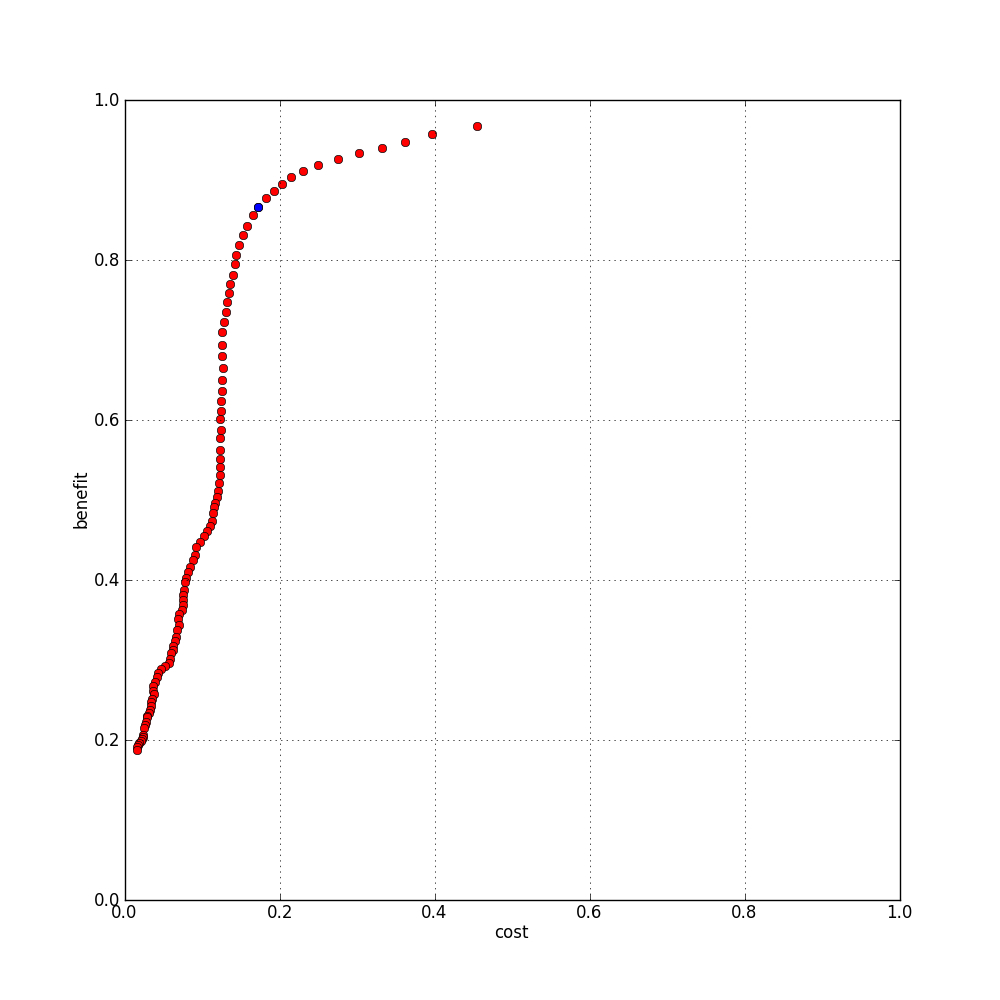
\includegraphics[width=0.75\textwidth]{img/2dcostbenefitexample2.jpg}
     \caption{An example of a 2D cost/benefit diagram, the blue configuration is the one with the lowest distance score}
\end{figure}
%
% \subsubsection{Testing RENAME}
% ANDERS
%
\subsection{Robustness}\label{sec:robustness}
%
On top of the ordinary parameter tuning and testing we also attempt to measure the overall robustness of each of the algorithms with respect to the change of parameter. This is done by calculating the area under the curve (AUC) of the cost/benefit diagrams generated by each algorithm. For this we use the entire dataset, which is to say that it happens after the 5-fold cross validation. Any algorithm, whos benefit-value is generally larger than its corresponding cost-value, across all choices of parameter(s) will have an AUC larger than 0.5. The larger the AUC is the more robust the algorithm is toward changes to its parameter(s). Since the points produced by most of the algorithms are not evenly spread over the entire diagram, we insert points at the (0,0) and (1,1) coordinate in order to cover the entire span of the diagram along the x-axis. It can be argued whether this is the most correct way to handle this, but it does produce comparable AUCs across all algorithms. Unlike the tweaking and testing described above this does not tell us anything useful about the best parameter to choose since we have no way of knowing how this would generalise. But it does tell us something about the nature of the algorithm itself. In general we would prefer our algorithm of choice to be as robust as possible as it signifies a sensible selection of parameters. 
%
\subsection{Multi-parameter algorithms}\label{sec:ph1multiparameter}
%
All our algorithms, except one, only have one parameter. This makes them easy to tweak and test and also very straightforward to generate cost/benefit diagrams for. The \textit{ICSM} algorithm, however, has two parameters and this causes some problems. First and foremost the additional parameter makes tweaking much more computational expensive. With the other algorithms we tweak the one parameter by one percentage point in each iteration, which limits the number of configuration to a hundred. To do so with the \textit{ICSM} algorithm would require 10.000 tweak iterations, which is much too expensive even when the results of intermediate calculations are cached on disk. In order to bring this number down we start we start out by attempting to learn something about the base characteristics of the algorithm by probing it using some uniformly selected configurations. In the case of the \textit{ICSM} algorithm we see that the \textit{contrast} parameter has a huge influence on how well the algorithm is defined in the cost/benefit spectrum. For very low values of \textit{contrast} almost all results are undefined because all frames are marked as good, which makes it impossible to calculate precision and recall correctly. On the other end of the spectrum, when \textit{contrast} is large, the effect of changing it is very small, signifying that it converges toward some optimal value. Based on this information we choose to decrease the precision with which we tweak \textit{contrast} to ten percentage points per iteration. This brings the total number of tweak iterations down to 1000. This still takes a long time, but it is manageable.\\
\\
The second problem is encountered when generating the cost/benefit diagrams and calculating the AUC. The effect of changing more than one variable is not illustrated very well in a two-dimensional cost/benefit diagram. The points, which really belong in a higher dimensional space, are flattened into the plane resulting in several curves without any clear connection to each other. This also causes problems when calculating the AUC for the algorithm, since curves generated by bad performing configurations can be hidden below curves generated by good performing ones, which in the end results in a over-optimistic robustness score.
%
% \begin{figure}
%      \centering
%      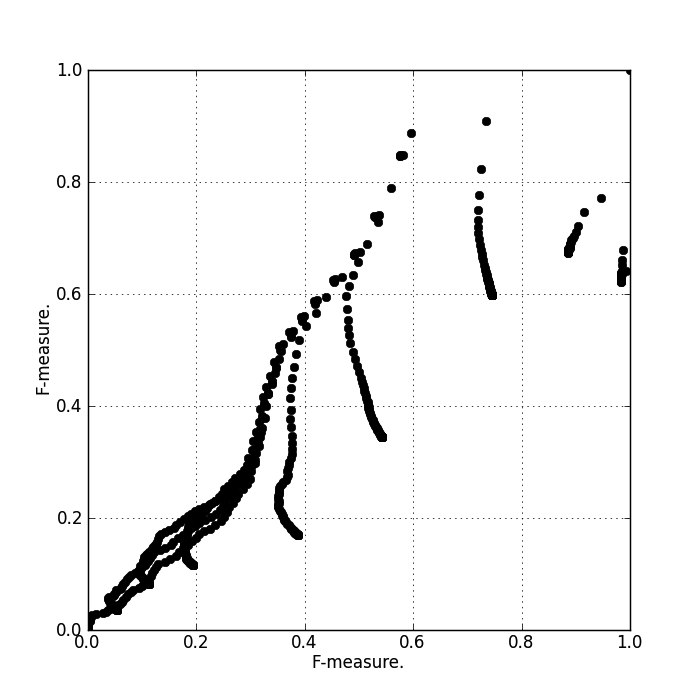
\includegraphics[width=0.75\textwidth]{img/2dcostbenefitexample.jpg}
%      \caption{An example of a 2D cost/benefit diagram for an algorithm with two variables}
% \end{figure}
%
%
% Noter fra Kim: Y-axis = benefit? X-axis=cost? Ser mærkeligt ud, drop!
%
In order to overcome this problem we simulate having only one parameter by locking the second one (contrast) to a specific value and then performing our analysis as usual. We repeat this over and over again, locking the contrast parameter to a new value in each iteration until we have covered all configuration combinations. For the robustness analysis we then add an aditional axis, representing the locked parameter, to our cost/benefit diagram and draw our points in three dimensions. The plane created illustrates the robustness of the algorithm much better. Since the choice of contrast values across all iterations are uniformly distributed, we can easily determine the AUC for the algorithm by simply calculating the individual AUCs for each selection of contrast value and compute an average.
%
\begin{figure}
     \centering
     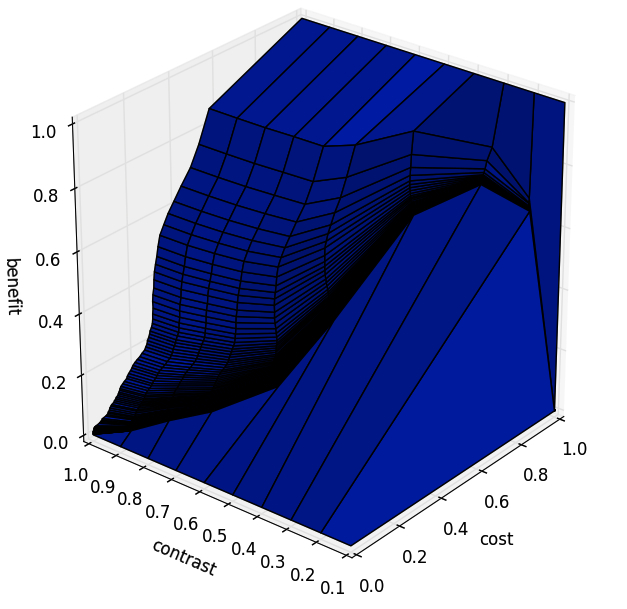
\includegraphics[width=0.75\textwidth]{img/3dcostbenefitexample.jpg}
     \caption{An example of a 3D cost/benefit diagram}
\end{figure}
%
% \subsubsection{Test cases}\label{sec:testcases}
%
\subsection{Frame by frame classification (FFC)}\label{sec:fbfclass}
%
The first test case only looks at each frame independently. For each frame we determine the level of contrast and the shift vector magnitude and use this information alone to perform a binary classification of the frame as \textit{good} or \textit{bad} using the algorithms described above. The results are compared with our \textit{gold standard} for the videos and the amount of true and false positives and negatives are used to calculate precision and recall for both classes.
%
\subsection{Temporal classification (TC)}\label{sec:tempclass}
%
In the second test case we change the way we punish misclassifications. We instead consider the videos as switching back and forth between two states, \textit{good} and \textit{bad}. Misclassifications, which happen close to these change-of-state's are punished less than those that happens elsewhere. The rationale behind this is that it is very difficult to objectively determine the exact point (frame) where a human observer will consider the quality of a video as changing from one state to the other. Likewise, we expect a human observer to ignore very short sub-parts of good or bad quality footage, if it is surrounded by a significant amount of footage of the opposite type. Overall, we want to be more tolerant of misclassifications, where it makes sense. For this we need a more advanced \textit{penalty function} than the simple binary check from the FFC test case.\\
%
We start by identifying all the positions in the sequence of frames where the state changes from good to bad or vice versa. Let $S$ be the set of all these positions. Also let $x$ any position in the video and let $c$ be some level of tolerance for mistakes. A \emph{penalty function} for determining the ratio of punishment for a misclassification at position $x$ is then defined as:
%
\begin{displaymath}
P(x) =1 - MAX_{s\in S}(e^{-\frac{(x-s)^{2}}{2c^{2}}})
\end{displaymath}
%
This function places a series of inverted gaussian bell curves at the point of every change of state. Figure \ref{fig:penaltycurve} shows an example of this. The value $c$ defines the width of the curve and thus determines how tolerant we are.
%
% Noter fra Kim: Valgt hvordan?
%
\begin{figure}
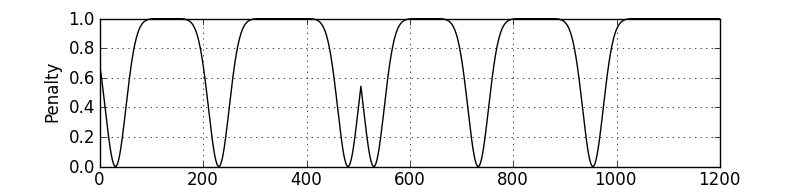
\includegraphics[width=1\textwidth]{img/penaltyfunction.jpg}
\caption{An illustration of a curve generated by the penalty function P}
\label{fig:penaltycurve}
\end{figure}
%
\emph{P(x)} always returns a value between 0 and 1, that tells us how severe a misclassification at position $x$ is. All correct classifications are treated just like in the FFC test case. However, if a misclassification occurs, we look at the \textit{penalty function} to see how the classification should be scored. There is one problem with this appraoch. It makes maintaining accurate true- and false- negative and positive values slightly less trivial. If a misclassification occurs at frame \textit{x} and \emph{P(x)} is very close to 0, how true (or false) is the classification)? The way we handle this is simply by adding \textit{P(x)} to the \textit{false} ratio for this type (positive or negative) and \textit{1 - P(X)} to the opposite type. That is, we quantify the classification as being both true and false to a varying degree determined by the \textit{penalty function}.
%
\subsection{Smoothing of the algorithm suggestions}\label{sec:classsmooth}
%
Finally, for both algorithms, we also investigate the effect of smoothing the classification results. This is done to remove outliers in the final results and should not be confused with the smoothing of the \textit{contrast} and \textit{shift vector magnitudes} in the algorithms themselves.
%
\subsection{Results}
% ANDERS
Table \ref{tab:algoconfigs} shows the different algorithm configurations. \textit{Label} is the specific algorithm configurations name. \textit{Algorithm} is the specific algorithm. \textit{Smoothness Degree} is a measure of how much the algorithm result is smoothed as described in \ref{sec:classsmooth}. \textit{Comparison Method} indicates if the algorithm result is compared using Frame-by-Frame Classification as described in section \ref{sec:fbfclass}, or using a Temporal Classification, as described in \ref{sec:tempclass}, using the stated \textit{Tolerance}. \textit{Parameter} is the parameter configuration for a given algorithm.\\
A final configuration of an algorithm is hence a smoothness degree for smoothing the resulting frame states and a set of parameters, and which method was used to tune this configuration in respect to the gold standard.\\
Algorithm configuration and configuration is used interchangeably in the following.
%The parameter is the average over the 5-fold cross validation. Smoothness degree describes how much the result is smoothed using triangular smoothing. The comparison method is either frame-by-frame (FFC) or temporal (TC), both described in section \ref{sec:testcases}.\\
%
\begin{table}[h]
  \begin{tabular}{| l | l | p{2cm} | p{2cm} | c | c | }\hline
    Label & Algorithm & Smoothness degree & Comparison method & Tolerance & Parameter(s)\\\hline
    ICSM1 & ICSM & 0 & FFC & N/A & (0.052, 0.720) \\\hline
    ICSM2 & ICSM & 12 & FFC & N/A & (0.054, 0.720) \\\hline
    ICSM3 & ICSM & 0 & TC & 24 & (0.060,0.720) \\\hline
    ICSM4 & ICSM & 0 & TC & 48 & (0.064,0.720) \\\hline
    ICSM5 & ICSM & 12 & TC & 24 & (0.058,0.720) \\\hline
    ICSM6 & ICSM & 12 & TC & 48 & (0.064, 0.720) \\\hline
    ICSM7 & ICSM & 0 & TC & 12 & (0.056, 0.720) \\\hline\hline
%
    CCSM1 & CCSM & 0 & FFC & N/A & 0.092 \\\hline
    CCSM2 & CCSM & 12 & FFC & N/A & 0.088 \\\hline
    CCSM3 & CCSM & 0 & TC & 24 & 0.100 \\\hline
    CCSM4 & CCSM & 0 & TC & 48 & 0.108 \\\hline
    CCSM5 & CCSM & 12 & TC & 24 & 0.094 \\\hline
    CCSM6 & CCSM & 12 & TC & 48 & 0.110 \\\hline
    CCSM7 & CCSM & 0 & TC & 12 & 0.098 \\\hline\hline
%
    CO1 & CO & 0 & FFC & N/A & 0.462 \\\hline
    CO2 & CO & 12 & FFC & N/A & 0.460 \\\hline
    CO3 & CO & 0 & TC & 24 & 0.466 \\\hline
    CO4 & CO & 0 & TC & 48 & 0.474 \\\hline
    CO5 & CO & 12 & TC & 24 & 0.468 \\\hline
    CO6 & CO & 12 & TC & 48 & 0.474 \\\hline
    CO7 & CO & 0 & TC & 12 & 0.466 \\\hline\hline
%
    SO1 & SO & 0 & FFC & N/A & 0.048 \\\hline
    SO2 & SO & 12 & FFC & N/A & 0.048 \\\hline
    SO3 & SO & 0 & TC & 24 & 0.056 \\\hline
    SO4 & SO & 0 & TC & 48 & 0.060 \\\hline
    SO5 & SO & 12 & TC & 24 & 0.056 \\\hline
    SO6 & SO & 12 & TC & 48 & 0.060 \\\hline
    SO7 & SO & 0 & TC & 12 & 0.054 \\\hline%\hline
%
    % $\text{CSM}^{3}1$ & $\text{CSM}^{3}$  & 0 & FFC & N/A & 0.366 \\\hline
    % $\text{CSM}^{3}2$ &$\text{CSM}^{3}$ & 12 & FFC & N/A & 0.366 \\\hline
    % $\text{CSM}^{3}3$ &$\text{CSM}^{3}$ & 0 & TC & 24 & 0.370 \\\hline
    % $\text{CSM}^{3}4$ &$\text{CSM}^{3}$ & 0 & TC & 48 & 0.388 \\\hline
    % $\text{CSM}^{3}5$ &$\text{CSM}^{3}$ & 12 & TC & 24 & 0.370 \\\hline
    % $\text{CSM}^{3}6$ &$\text{CSM}^{3}$ & 12 & TC & 48 & 0.382 \\\hline
    % $\text{CSM}^{3}7$ &$\text{CSM}^{3}$ & 0 & TC & 12 & 0.370 \\\hline
%
  \end{tabular}
\caption{Algorithm configurations}
\label{tab:algoconfigs}
\end{table}\\
%
Table \ref{tab:algoperf} shows performance of each algorithm configuration. As the parameters of each configuration is an average over a 5-fold cross validation \textit{Parameter(s) std. dev. \%} is a measure of how we expect the configuration to generalize to other data, where a low relative standard deviation indicates high generalizability, and a high relative standard deviation indicates a low generalizability. \textit{DS} is the distance score, describe in detail in section \ref{sec:ph1tweaking}, where a low score is achived if the algorithm configuration provided results close to the gold standard, and a high score is achived if the results was far from the gold standard. The distance score is an average over the 5-fold cross validation, and \textit{DS std. dev. \%} is hence again a measure of how the configuration generalize to other data. MÅSKE NOGET OM HVORFOR AT DETTE ER TILFÆLDET? \textit{AUC} is the Area Under the Curve, as described in \ref{sec:}, is only indirectly related to the specific configuration, as it is the result of all parameters tested during the tuning process. It gives an indication of how robust the algorithm performs.
%In Table \ref{tab:algoperf} the parameter(s) relative standard deviation is a measure of how much the parameter (is expected to) generalize to different data, where a low standard deviation equals a high level of generalization. The Distance Score (DS) is described in section \ref{sec:ph1tweaking}, and Area Under the Curve (AUC) is described in section \ref{sec:robustness}.\\
%
\begin{table}
  %\begin{tabular}{| l | p{2.5cm} |p{2.5cm} | p{2.5cm} | c |}\hline
  \begin{tabular}{| !l | ^p{2.5cm} | ^p{2.5cm} | ^p{2.5cm} | ^c |}\hline
    Label & Parameter(s) std. dev. \% & DS & DS std. dev. \% & AUC \\\hline
    ICSM1 & (7.7\%, 5.6\%) & 0.54 & 27.17\% & 0.51 (39.44\%) \\\hline
    CCSM1 & ~4.3\% & 0.54 & 27.90\% & 0.66 \\\hline
    CO1 & ~2.5\% & 0.81 & 28.10\% & 0.40 \\\hline
    SO1 & 15.6\% & 0.55 & 27.08\% & 0.65 \\\hline
    % $\text{CSM}^{3}1$ & ~2.2\% & 0.76 & 30.27\% & 0.44 \\\hline\hline
%
    ICSM2 & (14.8\%, 5.6\%) & 0.54 & 27.52\% & 0.51 (39.69\%) \\\hline
    CCSM2 & 19.6\% & 0.54 & 27.85\% & 0.67 \\\hline
    CO2 & ~2.4\% & 0.81 & 28.21\% & 0.40 \\\hline
    SO2 & 15.6\% & 0.54 & 27.54\% & 0.65 \\\hline
    % $\text{CSM}^{3}2$ & ~2.2\% & 0.76 & 30.87\% & 0.44 \\\hline\hline
%
    ICSM3 & (18.3\%, 5.6\%) & 0.29 & 31.10\% & 0.66 (41.71\%) \\\hline
    CCSM3 & 15.5\% & 0.30  & 34.30\% & 0.87  \\\hline
    CO3 & ~1.1\% & 0.50  & 28.73\% & 0.66 \\\hline
    SO3 & 14.3\% & 0.30  & 31.28\% & 0.86  \\\hline
    % $\text{CSM}^{3}3$ & ~0.0\% & 0.45  & 31.90\% & 0.70 \\\hline\hline
%
    ICSM4 & (15.9\%, 5.6\%) & 0.21 & 34.29\% & 0.70 (42.57\%) \\\hline
    CCSM4 & 17.0\% & 0.22 & 34.24\% & 0.92 \\\hline
    CO4 & ~2.9\% & 0.39 & 18.54\% & 0.79 \\\hline
    SO4 & 18.3\% & 0.22 & 35.54\% & 0.91 \\\hline
    % $\text{CSM}^{3}4$ & ~3.8\% & 0.36 & 20.37\% & 0.81 \\\hline\hline
%
    ICSM5 & (20.1\%, 5.6\%) & 0.29  & 32.02\% & 0.66 (41.78\%) \\\hline
    CCSM5 & 19.7\% & 0.30  & 33.81\% & 0.87  \\\hline
    CO5 & ~0.9\% & 0.49 & 28.31\% & 0.66 \\\hline
    SO5 & 14.3\% & 0.29 & 32.22\% & 0.86 \\\hline
    % $\text{CSM}^{3}5$ & ~0.0\% & 0.45 & 32.62\% & 0.70 \\\hline\hline
%
    ICSM6 & (15.9\%, 5.6\%) & 0.21 & 35.18\% & 0.70 (42.62\%) \\\hline
    CCSM6 & 19.1\% & 0.22 & 35.00\% & 0.92 \\\hline
    CO6 & ~2.9\% & 0.40 & 18.65\% & 0.79 \\\hline
    SO6 & 18.3\% & 0.22 & 36.61\% & 0.91 \\\hline
    % $\text{CSM}^{3}6$ & 18.3\% & 0.22 & 36.61\% & 0.91 \\\hline\hline
%
    ICSM7 & (14.3\%, 5.6\%) & 0.36 & 29.34\% & 0.62 (41.44\%) \\\hline
    \rowstyle{\bfseries}
    CCSM7 & 11.9\% & 0.36 & 31.71\% & 0.82 \\\hline
    CO7 & ~1.1\% & 0.60 & 26.18\% & 0.56 \\\hline
    SO7 & 14.8\% & 0.36 & 30.14\% & 0.81 \\\hline
    % $\text{CSM}^{3}7$ & ~0.0\% & 0.55 & 28.93\% & 0.60 \\\hline
%
  \end{tabular}
\caption{Algorithm performance}
\label{tab:algoperf}
\end{table}\\
%
Table \ref{tab:algoseq} shows some of the side effects of each configuration. \textit{GSL} is the Good Sequence Length which is a count of how many sequences of frame states that were classified as $1$, whereas \textit{BSL} is a count of how many sequences of frame states that were classified as $0$. A sequence is thus defined as a number of subsequent frames that share the same classification. The relative standard deviation of both GSL and BSL are computed, along with the longest GSL and BSL.
%In Table \ref{tab:algoseq} a Good Sequence Length (GSL) is the number of consecutive good frames, and a Bad Sequence Length (BSL) is the number of consecutive bad frames. Both measures is an average (over each test-set) and the relative standard deviation along with the longest GSL and BSL is also supplied in Table \ref{tab:algoseq}.
%
\begin{table}
  \begin{tabular}{| l | c | c | c | c | c | c |}\hline
  %\begin{tabular}{| !l | ^c | ^c | ^c | ^c | ^c | c |}\hline
    Label & GSL & GSL std. dev. \% & longest GSL & BSL & BSL std. dev. \% & longest BSL  \\\hline
    ICSM1 & 205 & 217\% & 5105 & 40 & 155\% & 536 \\\hline
    CCSM1 & 214 & 214\% & 5121 & 40 & 160\% & 607 \\\hline
    CO1 & 290 & 28\% & 11079 & 73 & 196\% & 1690 \\\hline
    SO1 & 198 & 221\% & 5105 & 40 & 157\% & 743 \\\hline
    % $\text{CSM}^{3}1$ & 264 & 326\% & 11078 & 69 & 204\% & 1691 \\\hline\hline
%
    ICSM2 & 248 & 199\% & 5115 & 47 & 152\% & 608 \\\hline
    CCSM2 &245 & 200\% & 5118 & 47 & 164\% & 739 \\\hline
    CO2 & 328 & 317\% & 11079 & 84 & 185\% & 1718 \\\hline
    SO2 & 231 & 206\% & 5115 & 47 & 170\% & 1087 \\\hline
    % $\text{CSM}^{3}2$ & 309 & 301\% & 11078 & 80 & 190\% & 1692 \\\hline\hline
%
    ICSM3 & 221 & 210\% & 5105 & 39 & 156\% & 509 \\\hline
    CCSM3 & 222 & 210\% & 5121 & 39 & 162\% & 607 \\\hline
    CO3 & 340 & 308\% & 11079 & 69 & 215\% & 1690 \\\hline
    SO3 & 209 & 214\% & 5105 & 38 & 147\% & 491 \\\hline
    % $\text{CSM}^{3}3$ & 319 & 298\% & 11078 & 66 & 223\% & 1691 \\\hline\hline
%
    ICSM4 & 229 & 209\% & 5122 & 39 & 149\% & 509 \\\hline
    CCSM4 & 225 & 213\% & 5123 & 38 & 154\% & 537 \\\hline
    CO4 & 378 & 316\% & 12080 & 71 & 217\% & 1690 \\\hline
    SO4 & 216 & 209\% & 5122 & 37 & 147\% & 482 \\\hline
    % $\text{CSM}^{3}4$ & 388 & 280\% & 12082 & 59 & 225\% & 1687 \\\hline\hline
%
    ICSM5 & 257 & 186\% & 5115 & 47 & 149\% & 608 \\\hline
    CCSM5 & 248 & 198\% & 5118 & 46 & 156\% & 739 \\\hline
    CO5 & 411 & 290\% & 11079 & 80 & 202\% & 1690 \\\hline
    SO5 & 246 & 200\% & 5115 & 45 & 143\% & 608 \\\hline
    % $\text{CSM}^{3}5$ & 364 & 280\% & 11078 & 75 & 211\% & 1692 \\\hline\hline
%
    ICSM6 & 266 & 198\% & 5122 & 45 & 144\% & 534 \\\hline
    CCSM6 & 260 & 200\% & 5129 & 45 & 142\% & 537 \\\hline
    CO6 & 431 & 298\% & 12080 & 82 & 201\% & 1690 \\\hline
    SO6 & 259 & 195\% & 5122 & 45 & 139\% & 482 \\\hline
    % $\text{CSM}^{3}6$ & 397 & 284\% & 12082 & 74 & 215\% & 1687 \\\hline\hline
%
    ICSM7 & 212 & 213\% & 5105 & 39 & 153\% & 510 \\\hline
    CCSM7 & 220 & 212\% & 5121 & 39 & 162\% & 607 \\\hline
    CO7 & 340 & 308\% & 11079 & 69 & 215\% & 1690 \\\hline
    SO7 & 208 & 214\% & 5105 & 39 & 149\% & 491 \\\hline
    % $\text{CSM}^{3}7$ & 319 & 298\% & 11078 & 66 & 223\% & 1691 \\\hline
  \end{tabular}
\caption{Sequence data}
\label{tab:algoseq}
\end{table}
%
\subsection{Analysis}
%
Table \ref{tab:algoperf} summarizes the primary results of our test, where the Distance Score is the primary attribute when rating the performance of a configuration. Note that each configuration uses either the Frame-by-Frame method, or the Temporal Classification method, when comparing against the golden standard. Configurations using different comparison methods are not directly compareable as the Frame-by-Frame method generally punishes errors harder than the Temporal Classification method. Configuration labels with a postfix of 1 or 2 uses the Frame-by-Frame comparison method, and labels with a postfix of 3 to 7 uses the Temporal Classification method.\\
The Distance Score standard deviation are all in the area of $25-35\%$ except some configurations of the Contrast Only algorithm. Both of these configurations uses the Temporal Classification method with a tolerance of 48 (the highest tested), and both has the worst score compared to other algorithms with compareable configurations.\\
We have marked the configuration with the best performance in Table \ref{tab:algoperf} with \textbf{bold}, namely CCSM7. It has a relatively low Distance Score by $0.36$ which is better than or equal to 15 out of 28 configurations. CCSM7 uses the Temporal Classification method with a the lowest tested tolerance, 12, and a smoothness degree of 0, ie. no smoothing, which means it will be punished greatly for any errors compared to most other configurations. CCSM7 also has a relatively large AUC which indicates that the algorithm itself is fairly robust. All other configurations of this algorithm also has a large AUC, supporting this assumption.\\
A close runners up is ICSM7 which had the same Distance Score as CCSM7. It is however not nearly as robust as CCSM7 which is due to some parameter configurations of the contrast ratio treshold produces very poor results.\\
The SO algorithms performs almost as well as the CCSM and ICSM algorithms, which leads us to believe that the camera movement is the defining attribute when estimating image quality. We do however only have a fairly limited amount of night-shots, and we expect that this is the edge that these two algorithms has over SO.\\
Table \ref{tab:algoseq} summarizes some of the side-effects of each configuration. Of note is that BSL is no more than 2 digits, they are all in the range $39-84$, for all configurations which tells us that sequences of poor footage are generally short. The longest BSL for CCSM7 is 607 frames (ca. 25 seconds) which tells us that there do exists longer sequences of bad footage, but this is certainly an extreme outlier (relative standard deviation is $167\%$).
Table \ref{tab:algoseq} also shows that there is on average 5 times more good footage than bad if we consider the results provided by CCSM7. It also finds a sequence of 5121 frames, roughly 3.5 minutes, which only supports this claim.\\
%
MEASURE HOW GOOD THE CCSM7 CONFIGURATION ACTUALLY WAS. IE. HOW MANY FRAMES DID IT GUESS CORRECTLY, AND HOW MANY DID IT GUESS WRONG.
%
% In general we have learned from these results that an algorithm that considers atleast camera movement in a video provides a significantly better assesment of the image quality than those that do not. 
%Table \ref{tab:algoperf} summarizes the primary results of our test. We cannot directly compare different configurations of the various algorithms as we expect a higher tolerance for error in some configurations, either by applying a gaussian filter (as described in Section [REFERENCE]) in the comparison method or triangular smoothing (as described in Section [REFERENCE]) of the result, or both.\\
%We therefore try to identify the configuration with the best performance mainly by comparing distance scores (low is better). Secondly the generalizability of a configuration is taken into account to break ties by looking at the relative standard deviation of the parameter(s).\\
% AUC is also mentioned in the table, but as it describes how sensitive an algorithm is to parameter-change...\\
% We did not expect the CO\textit{X} and $\text{CSM}^{3}\textit{X}$ algorithms to perform very well as the first does not take camera-movement into account, and the second ???????????????????????\\
% The 7th configuration does not apply triangular smoothing, and also uses a fairly low tolerance of 12 frames, roughly translated to a margin of error of half a second in each end of a sequence, yet it still achives a distance score of $0.36$ in 3 out of 5 algorithms and a relative standard deviation around $30\%$. We use the parameter relative standard deviation to break the tie where CCSM7 comes out on top. It also has the highest AUC, and we should therefore expect it to perform well even for other choices of parameters.\\
% The performance can generally be explained by the nature of our dataset, as there simply is very few frames where contrast is an issue. The higher relative standard deviation of SO7 could be explained by it trying to overcompensate in the few cases where a frame is classified as bad because of a low contrast.
%
\subsection{Risks and Limitations}
% LAUGE
In order to limit the scope of the testing and analysis phase we make some decisions which should be noted as a lot of areas related to determining the best algorithm and the optimal algorithm-parameter combination are left to be explored:\\
\\
All our algorithms square the \textit{contrast} and \textit{shift vector magnitude} values they come up with for each frame. The reason for this is that we want to increase their sensitivity toward bad values as compared to good ones. However, we have not done any real experimentation in this context and it is possible that a higher or lower power would yield better results. Furthermore we smooth these values across neighbouring frames in order to eliminate the worst outliers. It does not seem to have any significant effect on the final correctness of the algorithms, but this is neither an area in which we have done any real experimentation. Another important thing to remember is that we actually compute \textit{contrast} differently than Girgensohn et al.\cite{Girgensohn:2000:SAH:354401.354415}. Our method should be more robust toward very uniformly colored frames, but their original method could be more effective in general.\\
\\
When generating the cost and benefit scores we calculate the harmonic mean between the positive precision and the negative recall, as well as the positive recall and the negative precision, respectively. In our experimentation we have simply weighted the two values in each pair evenly, but it is possible that a skewed weighting in one or both of means would perform differently. It is even possible that this pair combination is not the right one for the task, although we argue that it intuitively makes sense.\\
\\
JEG MENER IKKE AT DET ER EN RISIKO/BEGRÆNSNING. MAN KAN ALTID TESTE FOR FLERE PARAMETRE (DER ER I TEORIEN UENDELIGT MANGE KOMBINATION). ANALYSEN ER LAVET PÅ BAGGRUND AF DE KONFIGURATIONER VI HAR TESTET. DET ER IKKE ET SPØRGSMÅL OM AT FINDE DEN BEDSTE OVERALL, MEN DEN BEDSTE AF DEM VI TESTER UDFRA NOGLE NOGENLUNDE FORNUFTIGE PARAMETRE.\\
In our experiment with smoothing the classification suggestions generated by the algorithm, in order to remove outliers, we restrict ourselves to only testing two different degrees of smoothing. More could be learned by experimenting with this value as an additional parameter of the algorithms. Informal testing did show little impact of a much higher degree of smoothing than the ones tested. \\
\\
The same can be said about the tolerance-value in the Temporal Classification. Exactly what degree of tolerance is the most reasonable is up for debate and any changes could, and probably would, change the outcome of our results.\\
\\
MAYBE THE 0 COST/MAX BENEFIT AND VICE VERSA. IS ONLY THEORETICALLY ACHIVEABLE, IE. THERE EXISTS NO PARAMETER CONFIGURATION THAT WILL ACHIVE THIS???\\
Also mentioned ealier, when calculating the AUC's for each algorithm we insert the points (0,0) (1,1) along with the points generated by the cost/benefit calculations in order to make sure each algorithm's curve cover the entire span of the x-axis. This has the effect of normalising the AUC around 0.5, which is useful for AUCs based on a curve that is only defined partly along the x-axis. It is however possible, that the very fact that a curve is not defined all along the x-axis is a sign of low robustness especially if the curve only is present near x = 1, that is, if the cost value is generally very high. If this is the case we risk ending up with invalid assumptions of robustness.\\
\\
In the \textit{ICSM} algorithm we chose to simplify our tweaking process by decreasing the precision on the second parameter, \textit{contrast}. The rationale for this is described in section~ \ref{sec:ph1multiparameter}. This means that our understanding of the influence of contrast in this algorithm is less detailed.\\
\\
Finally, it should be mentioned that all our tests are performed by treating the quality assessment problem as a task of binary classification. As described in section~ \ref{sec:videoclipsegmentation}, we are actually not interested in such a hard classification in the final system. Rather we want the quality of a region of video-footage to be expressed as a soft (un)suitability curve, from which we can make some general assumptions. However, the nature of our tests, especially the way in which we generate our gold standard (section~ \ref{sec:framequalityassessmentdataset}, requires us to simplify the problem into this binary form. Some of the aspects of the problem, which are lost by doing this, are to some extent accounted for, for example in the Temporal Classification test case, which allows for misclassifications to be treated in a more soft manner, but others are undeniably lost. This should also be taken into account, when considering the generalisability of our results.
%
\section{Summary}
%
We have explored different methods for estimating the image quality in video footage. Our approach focuses on the overall level of contrast in the individual frames as well as the movement of the camera. As our dataset includes relatively few night-shots we have not been able to confidently measure the importance of the contrast variable in the proposed methods. We do however have an indication of methods that considers contrast along with camera movement have an edge compared to methods that only looks on either of the two, where a method that considers only contrast performs poorly.\\
Our dataset is in general of high quality, as all data has been screened by a human before it was put on YouTube. Some of it has even been edited into a video that we later cut up and uses as raw footage. This has had an impact on our results as $X\%$ of the dataset was classified as a good frame by our gold standard.\\
The gold standard itself has an undefined margin of error. We never got around estimating just how error-prone it was to have a single person subjectively determine if a frame was good or bad. Informal testing did show some disagreement amongst the authors.
 %We have constructed, and testet, a set of algoritms, which uses these two variables to compute an unsuitability score for each frame in the videos. This score is then cast into the binary range using configurable threshold values. We compare the different algorithms 
%
% NEED TO WRITE ABOUT HOW THE LABELLER WORKS: THROWS AWAY SMALL SEGMENTS (< 6 FRAMES), MERGES NEARBY SEGMENTS, GENERALLY SMOOTHES DATA
%
% Remember to mention that video quality isn't used after phase 1 due to the side effects cased by labeling the video (namely that bad quality segments don't receive any labels). in a real world application this quality measure could be used to reduce the amount of data to analyze. This should probably be in the discussion section or the summary section for this phase.
%
% Contrast metadata er faktisk aldrig brugt, er det?
%
\chapter{Grouping and labeling}
%
Grouping and labeling comes down to extracting information about what is happening in a piece of video footage. We want to be able to distinguish between different \textit{types} of scenes so we have a way to structure the final video summaries. We want to be able to define a sequence of different scene types that should be put together.
%
\section{Literature Study}
%
There are many ways to extract context from images, sound and video. Some focus on the depicted scene itself, while others look at the events happening in the scene. Location and time of day would be an example of the former while elements such as excitement, violence and other specific behaviour are examples of the later.\\
Hanjalic, A. \cite{citeulike:405480} describes a way to identify regions of high levels of excitement in sports videos based on a manually selected set of features. These features can be both visual (e.g. movement in an image or change of camera position) or audial (based on the energy contained in the audio track).\\
Optical Flow, as described by Bouguet \cite{Bouguet2000}, can also be used to detect events or objects in video. Optical Flow analyses changes in the intensity pattern in images. In many cases this indirectly indicate changes in the 3D scene caused by moving objects or a change of view-point. [REFS] describes ways to identify certain types of actions occuring within videos, such as violent behaviour and [REF] looks at general crowd movement in public places.\\
% Lauge: Der skal skrives lidt mere til disse artikler.
Reisman et al. \cite{CrowdDetectionInVideoSequences} describes a way to identify crowds of pedestrians from a moving vehicle by detecting inward moving optical flow. I.e. flow which is highly likely to be caused by moving objects and not a change of view-point.\\
Arandjelović \cite{Arandjelovic08crowddetection} attempts to identify crowded regions in still images based on the hypothesis that crowds contain a certain general structure, namely that an image with crowds in it will contain regions, which at a close scale resembles individual people, while at a larger scale will contain repetative structures.\\
% Lauge: Flere crowd detection artikler?
Zhong et al. \cite{10.1109/CVPR.2004.78} describes a technique for unsupervised detection of unusual events in a video stream. The entire stream is divided into overlapping 4 second segments from which an overall movement pattern is established. Individual segments that differ too much from this patter are considered unusual.\\
% Lauge: Day/Night article her skal uddybes og omskrives:
In [REF] the authors describe how to classify still images through a hierachy of Support Vector Machines, including day/night classification.\\
% Lauge: Jeg har rykket Haar Cascade classifier ned i sit eget afsnit under Method, men måske skal vi lige have en enkelt linje om det her
Angin et. al \cite{10.1109/MDM.2010.71} describes a method of automatically detecting the color of traffic lights. % Lauge: Vi skal lige have læst/skrevet lidt mere om denne og evt. relation til police blinker detecion
%
\section{Method}
%
The labeling happens in two phases. First we extract different kinds of metadata from the individual videos. This is done frame-by-frame, for each type of metadata, so we end up with a collection of describing properties throughout each video. Some of the metadata is directly available from the earlier phases of the project. The level of \textit{contrast} and the \textit{shift vector magnitudes} described in section \ref{} and revisited below in sections \ref{sec:contrastdata} and \ref{sec:svmdata}, are examples of this. We use the frame mean pixel intentisity to estimate overall brightness (section \ref{sec:brightnessdata}) and seperate the blue color channel (section \ref{sec:blue_channel}). People detection (section \ref{sec:peopledata}) is done using Haar cascade classifiers and Optical flow (section \ref{sec:opticalflowdata}) is used for extracting additional event information.\\
\\
The actual labeling is subsequently done by analysing the metadata in a collection of classifiers. Section \ref{sec:police_detection} describes a \textit{police blinker} classifier, which searches for oscillation in the blue channel from the individual frames. Section \ref{sec:overviewclassifier} describes an \textit{overview} classifier, which attempts to detect footage containing litle egomotion (camera movement). In section \ref{sec:verticaloscillationclassifier} we attempt to identify vertical oscillating movement in the optical flow, using it as an indicator for people jumping or signs being lifted into the air. Section \ref{sec:incrowd} describes an \textit{in-crowd} classifier, which uses facial- and person- detection to detect footage with several people in it. In section \ref{sec:infocus} we further explore the area of people detection, by looking for footage, which focuses on a specific (assumably interesting) person for a duration of time. Finally, in section \ref{sec:daynightclassifier} we look at differentiating between day- and night- time footage by working with the different brightness and color intensity metadata we have extracted.
%
\subsection{Haar Cascade Classifier}\label{sec:hcc}
%
The Haar Cascade Classifiers (HCC)\cite{viola01,lienhart01,schmidt01,schmidt02} is an efficient tool for facial detection. It uses a data-structure called an integral image, an algorithm based on AdaBoost that selects critical visual features, and a method that combines complex classifiers to compute on the most promising object-like regions. Initial results by Viola\cite{viola01} achives 15 frames per second detection in an 384 by 288 pixel image using, by todays standards, outdated hardware.\\
%
An integral image (aka. summed area table) is a matrix where any point $(x,y$ is the sum of all pixels above and to the left of $(x,y)$ illustrated in Figure \ref{fig:integral_img} where $\square ABCD$ can be computed as $C-(D+B)+A$, ie. the sum of any subpart of the integral image can be quickly determined. Not only is the computation of this matrix efficient as a function of its nature (it can reuse already computed sums when building the matrix), the sum at any given point can be computed in constant time as it can be done by 4 lookups in the matrix followed by 4 additions/substractions.
%
\begin{figure}[!ht]
     \centering
     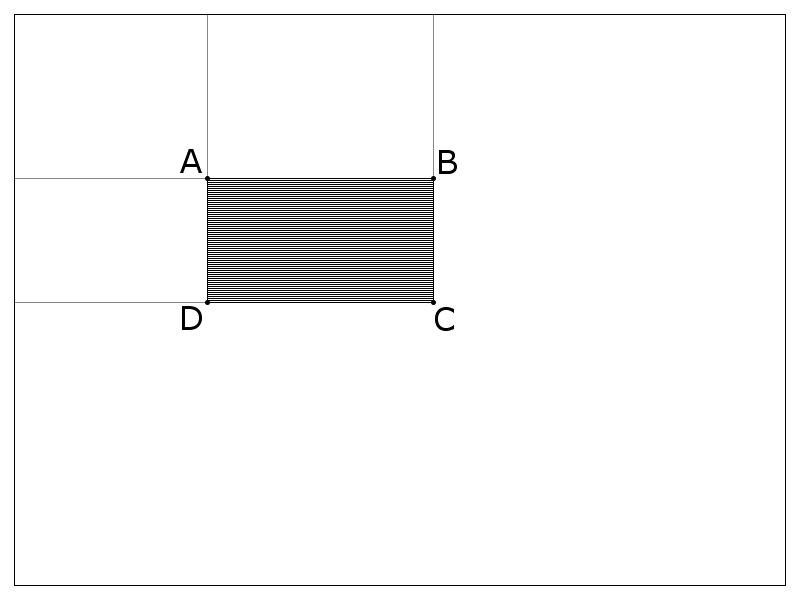
\includegraphics[width=0.50\textwidth]{img/integral_image.png}
     \caption{Integral image}\label{fig:integral_img}
\end{figure}\\
%
AdaBoost (Adaptive Boosting) is a meta-algorithm for boosting machine learning algorithms where subsequent classifiers built are tweaked in favor of those instances misclassified by previous classifiers. The derivative algorithm is a modification of AdaBoost that constrains each returned (weak) classifier to be dependent only on a single feature, which in turn is deemed a critical feature.\\
A method of using less complex processing to detect promising regions, and then apply the more complex processing on these regions.
%
\subsection{Metadata}
%
This section describes the different type of metadata we extract.
%
\subsubsection{Contrast}\label{sec:contrastdata}
%
The \textit{contrast} in a frame is defined as being the standard deviation of the intensity values in the image-matrix. This is described in detail in section \ref{}. A small deviation would indicate little contrast/diversity in color-intensity, and a large deviation would indicate a high contrast/much diversity in intensity. The \textit{contrast} metadata for each video consist of the set of these standard deviations for each frame.
%
\subsubsection{Shift vector magnitude}\label{sec:svmdata}
%
Like the contrast, the \textit{shift vector magnitudes} for each video is already computed as a part of the initial image quality assessment, as described in section \ref{}. We make a rough estimation of the egomotion (camera movement) by shifting all pairs of neighbouring frames until they more or less alligns up. This shift is expressed as a vector, whos magnitude tells us how much the camera is moving/shaking at each frame point in the video. The \textit{shift vector magnitude} metadata consists of set of these magnitudes throughout the video. It is used in the \textit{overview} classifier described in section \ref{sec:overviewclassifier}
%
\subsubsection{Brightness}\label{sec:brightnessdata}
%
The \textit{brightness} metadata consists of the mean pixel intensity in each frame throughout the video. It is used in the \textit{day/night} classifier described in section \ref{sec:daynightclassifier}.
%
\subsubsection{Blue color channel}\label{sec:blue_channel}
%
This particular type of metadata is extracted from the original videos (before grayscale conversion). Each frame in a video consists of a matrix of pixels in 3 channels; red, green, and blue. We extract the blue channel for the purpose of police blinker detection, described in detail in section \ref{sec:police_detection}, and day/night detection, described in detail in section \ref{sec:daynightclassifier}.
%
\subsubsection{The presence of people}\label{sec:peopledata}
%
Detecting the presence of people will help us determine if footage was recorded from within a crowd, described in detail in section \ref{sec:incrowd}, or if the footage has focus on a specific person, described in detail in section \ref{sec:infocus}, which indicates that this person is of special interest, ex. a speaker.\\
%
OpenCV provides a python-implementation of an already trained Haar Cascade Classifier, as described in section \ref{sec:hcc}, manifested as a range of xml-files describing the Haar like features of a human face, both front and profile, aswell as upper body, lower body, and full body.\\
By deploying facial detection to every frame in each video we get a good estimate of how many people are present, and also their location within each frame. This estimate is limited by the quality of the frame, ie. shaky video-clips have a reduced detection rate.\\
For the sake of simplicity we have not implemented the optimization of only analayzing select frames (ex. every third frame) which we do not believe will have a significant impact on the detection rate as we interpolate the detected objects between frames already.\\
We suggest that further optimizations involve exploiting the ready-at-hand metadata such as the general frame quality which severely impacts facial detection rates in a negative fashion.\\
Further optimization can be achived by exploiting the temporal data. Ie. instead of analyzing the entire frame by expanding the search window incrementally, we utilize knowledge of where people were present in the previous frame. This would require a customized HCC which is a major increase in complexity compared to the other mentioned optimizations.
%
MOVE TO RESULTS:\\
we also experienced a significant increase in false positives for banners and flags (which there is a presence well above normal in our training set). We are working with 480 by 640 pixel images and are able to achieve real-time facial detection (working on video with 24 frames per second).\\
%
\subsubsection{Optical Flow}\label{sec:opticalflowdata}
%
\paragraph{Optical Flow - Hvordan virker lortet?}
%
For in-frame event extraction we use optical flow \cite{Bouguet2000}.
%
% Lauge: Her skal skrives noget om hvordan optical flow (Lucas Kanade, artiklen ovenfor) fungerer
%
Unfortunately, most of the existing work done on both event- and crowd- classification focuses on settings with stationary cameras. Although Reisman et al. \cite{CrowdDetectionInVideoSequences} \textit{do} work with images from a camera fixed on a moving vehicle, their appraoch is still not applicable to our scenario, since our videos are recorded mostly by handheld devices, whose movement are a lot less predictable.\\
%
\paragraph{Optical Flow - Hvad gør vi?}
%
Where \textit{shift vector magnitudes} tells us something about how the camera itself moves, optical flow attempts to explain how the content within each frame moves. There has been a substancial amount of research put into this field. Most of our footage is recorded by handheld cameras often under very poor conditions. Extracting the optical flow of our videos is therefore not only a matter of analysing how reference points move around in the frame. First we must estimate the \textit{egomotion} (the motion of the camera) itself, in order to \textit{stabilise} the frame.
%
\paragraph{Frame stabilisation}
%
There are several ways to do this. An option is to use the \textit{shift vector magnitudes} that we have already computed. This intuitively makes sense since they are suppose to describe the movement of the camera at at each frame in the video. However, it turns out that although this data may be suitable for describing the general type of cameara movement (shaking, panning), especially when the data is smoothed across several frames, it has a relatively high margin of error for individual frames. This is especially the case if the camera moves very fast or if there actually \textit{is} a lot of movement within the frame. Another option is use the mean of all the optical flow vectors as the egomotion. Alternatively one could use the most commonly occuring vector. However, our experimentation showed that these two methods suffer from one serious limitation. If moving objects in the frame are very close to the camera, they tend to become more influencial than the stationary background and they end up swapping roles. The egomotion is then based on the movement of the large object, the opposite of what we want. The border-case for this condition is especially problematic. This occurs when a moving object takes up half of the frame. Often, changes in position will then \textit{periodically} cause it to be more or less dominant than the background. In these cases the egomotion vector will jump from one extreme to the other, in close succession, and thus become completely useless.\\
Some of these problems could probably be alleviated through further analysis or averaging across time. However, through our experimentation we came up with an approach that seems more promising.\\
\\
\textit{Corner detection} refers to identifying features in a frame, which are \textit{good to track}. They are areas (or points), which are likely to be clearly distinguishable on the following frames. This is often done by locating areas with low \textit{self simmilarity}. That is, areas that do not look like other areas close by. We found that generally, these points has a tendency to be present in stationary objects in the frame far more often than in moving objects, and thus form a very decent base for our egomotion vector. The implementation we use to identify these features is based on the Shi-Tomasi corner detection algorithm described by Shi et al. \cite{Shi_1994_3266}. We track these features and define our egomotion to be the mean of all the resulting displacement vectors.\\\\
%
Note: We have later come across other, more advanced techniques for calculating the egomotion of a video. Raudies et al. \cite{Raudies:2009:ELM:1612122.1612125} describes such a method. Unfortunately, do to our late discovery of this method we have not been able to test it.
% Lauge: Der skal skrives noget mere om denne metode, hvis den skal nævnes, desuden skal dette rykkes til future work
%
\paragraph{Detecting movement}
%
We now look at the movement within the frames. We do this by placing a grid of points across the frame and perform optical flow analysis on them. We use a pyramidal implementation of the Lucas Kanade feature tracker described by Bouguet \cite{Bouguet2000}.
% Flyt til parameter tuning:
We do the analysis with a grid of 24x16 points, using a search window of 30x30 pixels through two iterations.\\% TODO: ACTUALLY UNDERSTAND THIS and describe it here!!!
%
Some of the resulting vectors are considered invalid if we are unable to track them. This is often the case with points in the sky or in surfaces without any distinct features) or if the point being tracked ends up outside of the subsequent frame. Let $E$ be our egomotion vector. Then, for every vector $v \in V$, where $V$ is the set of valid displacement vectors, the isolated movement vector $v'$ is defined as:
\begin{equation}
v' = v - E
\end{equation}
Let $V'$ describe the set of all isolated movement vectors $v'$. $V'$ then describes the movement of objects within the frames.\\
Each vector $v' \in V'$ describes the movement of one particular point in the original grid. By looking at the different directions of flow we may be able to say something about what is going on in the video. To simplify the data we divide the optical flow vectors up into nine segments as shown in figure \ref{fig:opticalflow}. We calculate the mean of the movement vectors in each group, seperately, and use these nine new vectors to describe the overall flow in different parts of the frame.
%
% Lauge: RISK - This model may be too simple, for good results
%
\begin{figure}
     \centering
     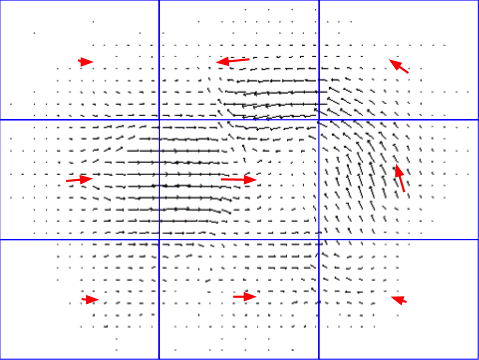
\includegraphics[width=0.75\textwidth]{img/optical_flow.png}
     \caption{Example of optical flow vectors in a frame. The red arrows shows the overall flow within a segment of the frame}\label{fig:opticalflow}
\end{figure}
%
The \textit{optical flow} metadata consist of sets of these nine vectors, calculated for each frame in the video. It is used in the \textit{vertical oscillation} classifier described in secion \ref{sec:verticaloscillationclassifier}.
%
%
%
%
%
\subsection{Label classifiers}
%
Each classifier performs a binary classifaction on a specific label. It analyses all the available footage and returns a collection of indexes to all the segments where it believs the specific label it to be present. These indexes consist of a reference to the video in question, as well as a start and end index. Depending on the classifier, these segments are then post-processed using \textit{segment interpolation} and/or \textit{segment smoothing}
%
\subsubsection{Segment Interpolation}\label{sec:labelmerge}
%
% Lauge: Denne sektion skal skrives om. Den giver ikke meget mening som den er. Desuden skal der skrives noget om 'truncation' som bliver refereret til flere steder senere
%
Segments in a video is easilly fragmented and two segments with the same label just a single frame apart will by all means and purposes be interpreted as such. This is often a result of fragmented metadata, ex. several consequtive frames with people present that our people presence detection algorithm failed to detect. To patch this fault we interpolate the segments by applying the label, $l$, to the frames between segment $a$ and segment $b$ if these are not too far apart (by default 24 frames) and both segments share the same label, $l$. As we are already analyzing segments we also filter out segments of diminutive length, which by default is 5 seconds.
%
\subsubsection{Segment Smoothing}\label{sec:labelsmooth}
%
% Lauge: Denne sektion skal skrives om. Den giver ikke meget mening som den er. Desuden skal der skrives noget om 'truncation' som bliver refereret til flere steder senere
%
If segments are higly fragmented because the label-algorithm that produced them made no attempt to smooth the frames and their respective label (or absence of same) we apply triangle smoothing on the segments, defaulting to a degree of $36$ frames equal to $1.5s$, and subsequently cut off values below a certain treshold, defaulting to $1/3$, ie. values below the treshold are truncated to $0$.
%
\subsubsection{Police Blinker classifier}\label{sec:police_detection}
%
By investigating the blue channel mean of each frame (section \ref{sec:blue_channel}) we are able to detect if the police blinker lights are present in part of a video.% Resultat
We analyze the blue channel mean as a function of time, and if these values are oscillating within certain parameters,% Specific frequency
we have an indication of the precense police blinker lights.
%
\begin{figure}[!ht]
     \centering
     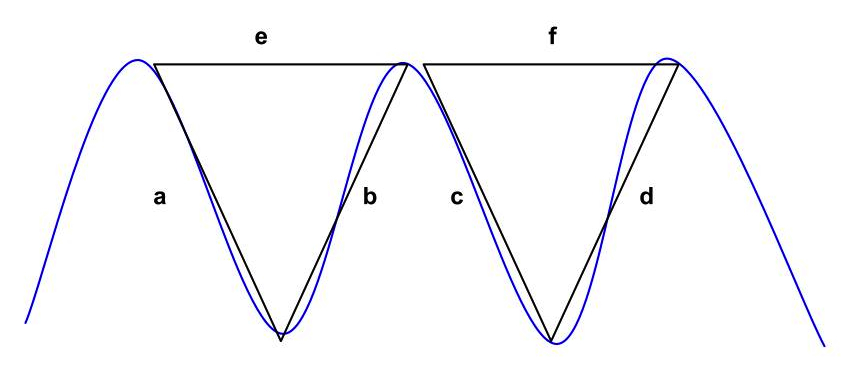
\includegraphics[width=1.05\textwidth]{img/triangles.jpg}
     \caption{}\label{fig:triangles}
\end{figure}\\
% Lauge: Mangler title + Lav rigtig figur
Local minima/maxima in an oscillating graph connected by straight lines will form triangular shapes as illustrated in Figure \ref{fig:triangles}, where consequtive triangles of roughly equal size indicate a steady oscillation. As an alternative to computing the area of each triangle we investigate how the length of the vertices in each triangle deviate from each other
\[
\text{std}([\|a\|,\|b\|,\|c\|,\|d\|]) < \tau_1,
\]
% a,b,c, og d skal defineres i tekst
for some threshold $\tau_1$ where std is the standard deviation. Analogously for the horizontal vertices
\[
\text{std}([\|e\|,\|f\|]) < \tau_2,
\]
% e og f skal defineres i tekst
for some threshold $\tau_2$.\\
The blue channel mean is smoothed using triangle smoothing with a degree of 5% paramter tuning
as this give softer curves on the graph. Oscillating segments are then detected, and nearby segments are merged as described in section \ref{sec:labelmerge} where segments up to 48 frames% paramter tuning
 apart are interpolated into a single segment, and segments shorter than 24 frames% paramter tuning
  are removed.
%
\subsubsection{Person in Focus classifier}\label{sec:infocus}
%
We compute a moving average (over 4 frames ~ 166ms)% paramter tuning
of the people presence metadata but excluding objects detected (partially) outside a centered bounding box.
% Lauge: Det er ikke klart hvad vi prøver at sige her:
A moving average of only 4 frames requires a low frequency of false negatives between frames which in turn makes a greater demand on the quality of each frame (steady or no camera movement, a good shot angle, and little background clutter). The frames and their respective label are smoothed as described in section \ref{sec:labelsmooth} with a smoothness degree of 36,% paramter tuning
equal to $1.5$ seconds, and a truncation value of $1/3$.% paramter tuning
 Nearby segments are merged as described in section \ref{sec:labelmerge} where segments up to 24% paramter tuning
  frames apart are interpolated into a single segment, and segments shorter than 120% paramter tuning
  frames, equal to 5 seconds, are removed.
%
%
\subsubsection{Overview classifier}\label{sec:overviewclassifier}
%
The \textit{overview} classifier attempts to detect footage with negligible egomotion, as well as little internal movement within the frames. Furthermore, in order to avoid overlap with the \textit{person in focus} footage, which often also holds these charactetistics, we also require the overview footage to not focus on any person in particular. The overview classifier uses the \textit{support vector magnitude} metadata described in section \ref{sec:svmdata}, the \textit{optical flow} metadata described in section \ref{sec:opticalflowdata}, as well as the actual labels classified by the \textit{person in focus} classifier described in section \ref{sec:infocus}.\\
We perform a slight triangular smoothing on the metadata in order to remove outliers. We also discard all footage, which has already been classified with the \textit{person in focus} label.\\
% RISK: One label takes precedence over another (not isolated)
We now look at the amount of movement in each part of the image in order to determine if a frame contain too much internal movement. Let the internal movement in a frame be defined as $f_{i} = [m_{1},m_{2} \dots m_{9}]$, where $m_{x}$ is the distance of movement occuring in a specific part the frame, calculated as the mean of the magnitude of all adjusted optical flow vectors, in an area. The number of areas exceeding a given limit, $s$, is then defined as:
%
\begin{equation}
A_{f} = \sum_{i=1}^{9}
\begin{cases}
0 & \text{, if } m_{i} \leq s\\
1 &  \text{, otherwise}
\end{cases}
\end{equation}
%
This way of analysing sub-parts of the image should improve the chance of detecting local charactaristics, which would be lost in an overall analysis of the frame. %Flyt til metadata afsnit?
 Next we combine this meassure with the egomotion in the frame, defined as $f_{e}$. The binary \textit{overview} classification of a frame is defined as:
\begin{equation}
O(f) =
\begin{cases}
0 & \text{, if } A_{f} > t \vee f_{e} > u \\
1 &  \text{, otherwise}
\end{cases},
\end{equation}
where $t$ is a threshold that defines how many areas are allowed to contain too much internal movement, and $u$ is a threshold defining the maximimum \textit{shift vector magnitude} we accept for the frame.
%
\subsubsection{Vertical Oscillation classifier}\label{sec:verticaloscillationclassifier}
%
The \textit{vertical oscillation} classifier attempts to detect footage with vertical movement of objects. Such movement can be caused by people jumping, by people gesticulating heavily whilst talking, or if people are raising signs into the air. In order to do this we look at the variance of the vertical direction of the optical flow vectors over some time.\\
As with the \textit{overview} classifier we analyse the internal movement in different areas of the image, in order to detect local charactaristics. Let $m \in M$ be the vertical movement in an area of a frame, calculated as the mean of the vertical movement of the adjusted optical flow vectors, in that area. Let $M$ be the set of all $m$. The variance in vertical movement in an area of the image, at a point $x$, is then defined as:
%
\begin{equation}
v(x) = std(\bigcup_{i=x-s}^{x} M_{i}),
\end{equation}
%
where $s$ is the timespan over which we want to calculate the variance. For simplicity we omit the case where $x \leq s$. In that case we let $V_{x} = 0$.\\
Let $V$ be the set of all nine $v$ throughout a video. The number of areas, in a frame $f$, in which vertical oscillation occurs is then defined as:
%
\begin{equation}
A_{f} = \sum_{i=1}^{9}
\begin{cases}
0 & \text{, if } V_{i}(f) < s\\
1 &  \text{, otherwise}
\end{cases}
\end{equation},
%
where $s$ is some threshold defining the minimum level of variance. The \textit{vertical oscillation} classification of a frame is then defined as:
%
\begin{equation}
V(f) =
\begin{cases}
0 & \text{, if } A_{f} < t\\
1 &  \text{, otherwise}
\end{cases},
\end{equation},
%
where $t$ is a threshold defining the minimum number of areas in which vertical oscillation must occur.
%
% RISKS: (zooming), maybe wrong method
%
\subsubsection{In-Crowd classifier}\label{sec:incrowd}
%
% Dette skal omskrives og rykkes rundt således at meget af det kommer ned i parameter tuning.
We compute a moving average (over 12 frames/500ms) of the people presence metadata to determine if the frame is shot from within a crowd, or slightly overlooking a crowd. If more than 1 person is present in the frame the frame is deemed to be \textit{in crowd}. Obviously 2 people does not make a crowd, but taking into account the high frequency of false negatives both in and between frames, this shows to provide a good estimate. The frames and their respective label are smoothed as described in section \ref{sec:labelsmooth} with a smoothness degree of 24, equal to 1 second, and a truncation value of $0.9$. Nearby segments are merged as described in section \ref{sec:labelmerge} where segments up to 24 frames apart are interpolated into a single segment, and segments shorter than 60 frames, equal to $2.5$ seconds, are removed.\\
A fallacy in this method are cases of just two people in a frame which are easily detectable, ie. facing a steady camera with no background clutter.\\
%
\subsubsection{Day \& Night classifier}\label{sec:daynightclassifier}
%
Night footage is not only darker than footage recorded during the day. It also contains significantly less blue color, which is the reason it often has a brownish or red tint. Our \textit{day/night} classifier analyses both the \textit{blue channel} metadata (described in section \ref{sec:blue_channel}) and the \textit{brightness} metadata (described in section \ref{sec:brightnessdata}).\\
First, we look at the correlation between the blue color channel and the overall brightness. Let $i$ be the frame position in the video, and let $R$ and $L$ be the set of brightness- and \textit{blueness}- values for all frames, respectively. Then the correlation $c_{i}$ is defined as:\\
%
\begin{equation}
c_{i} = \frac{L_{i}}{R_{i}} - 1
\end{equation}
%
A value above zero shows that blue is a dominant color in the frame. $c$ is therefor an indication of what type of footage we are dealing with.\\
Next, we look at the general distribution of brightness intensities throughout the video. We start by creating a histogram of the brightness distribution across the entire video. The histograms have a range of [0:255] and contain 10 bins of equal size. For each frame in the video, the mean brightness value is inserted into the histogram. Figure [FIG:REF] shows an example of this mapping.
%
[FIGURE]
%
Now we look at this histrogram and compare the mass of the partitions representing the darker frames with the mass of those representing the brighter ones. Let $H$ be the histogram for a video, and let $m\in [1..10]$ be some delimeter value. An indication of daytime is then defined as:
%
\begin{equation}
D = \sum_{i=1}^{m}H_{i} < \sum_{j=m+1}^{10}H_{j}
\end{equation}
%
Finally, let $C$ be the mean of all $c$ in a video. Our \textit{day/night} classifier is then defined as:
\begin{equation}
S =
\begin{cases}
\text{day} & \text{, if } C > 0 \vee D \\
\text{night} &  \text{, otherwise}
\end{cases}
\end{equation}
%
% \section{Dataset}
% %
% Here we should have a brief explanation of what videos are in our dataset.
%
\section{Findings}
%
This section describes the parameter tuning of the classifiers along with some informal performance statistics. In general all tuning is done through emperical testing. These parameters should therefore only be seen as a starting point for more extensive research. Unless otherwise noted, tuning is done on a small subset of the dataset. The entire dataset consists of 131617 frames ($\sim$ 90 minutes) of footage. For all, but the \textit{day/night} classifier, performance is meassured only in true positives/false positives. We derive the results from manual observation of the classified segments, where each classification is determined to be either correct or wrong.
%
\subsection{Police Blinker classifier}
%
...\\
\\
We meassure performance based on how many of the classified segments contain police blinkers or actually has police personal present in the footage. We include the latter scenario because the light from police blinkers off-screen may be detectable in the blue color channel, even if it is not visible to the human eye.\\
Out of the total $\sim$ 90 minutes of footage 699 frames $\sim$ 30 seconds are classified positive. Of this $\sim$ 65\% are what we consider \textit{true positives}. % Lidt her om false positives. Hvad er grunden til dem?
%
\subsection{Person in Focus classifier}
%
..\\
\\
We meassure performance based on how many of the classified segments has a specific person in focus. Segments with several people or crowds are considered incorrectly classified.\\
Almost 21 minutes of the entire dataset is classified as containing a person in focus. Hereof we consider $\sim$ 90\% to be \textit{true positives}.
%
\subsection{Overview classifier}
%
The \textit{overview} classifier (described in section \ref{sec:overviewclassifier}) analyses both the internal movement in the frames, as well as the overall egomotion of the camera.\\
The classifier has three thresholds, $s$, $t$ and $u$. $s$ is the maximum internal movement allowed in an area. $t$ is the maximum number of areas, which are allowed to break this limit, and $u$ is the maximum allowed egomotion for the entire frame.\\
The parameter tuning was done a small subset of the dataset, consisting of a handful of videos. Setting $s = 2 \text{ pixels}$ and $t = 2 \text{ areas}$, seems to ensure sufficiently low levels of internal movement. Setting $u = 10 \text{ pixels}$ appears to keep unsteady camera movement at a minimum, while still allowing for panoramic movement, which we do not want to discard.\\
Lastly, for the triangular smoothing of the metadata a triangle width of 120 frames is used. We have not performed any tuning on this parameter.\\
\\
It is difficult to exactly define what an \textit{overview} clip is. These are the charactaristics we look after when determining performance:
%
\begin{itemize}
	\item \textbf{Detachment from events}: The camera is not affected by the events being filmed. The camera is not affecting the events.
	\item \textbf{Scene depiction}: The footage shows the scene itself, not specific events in the scene. For this reason we do not accept footage of persons in focus.
	\item \textbf{Quality of footage}: The footage actually shows something. Footage depicting the sky or a close up shot of someones back, is not accepted.
\end{itemize}
%
As a rule of thumb, we consider segments fulfulling these requirements \textit{true positives}. In total $\sim$ 22 minutes are classified as being . Of these $\sim$ 43\% are considered correct. When reviewing the segments we clearly see that a lot of the \textit{false positives} are caused by clips with a \textit{person in focus}. This is a clear indication that our attempt to mutually exclude the two labels is failing.
%
\subsection{Vertical Oscillation classifier}
%
The \textit{vertical oscillation} classifier (described in section \ref{sec:verticaloscillationclassifier}) analyses the internal movement in the frames.\\
It has three thresholds. $v$ defines the area over which the standard deviation in vertical movement is calculated. $s$ defines the minimum level of variance accepted as vertical oscillation. $t$ defines the number of areas in the frame in which vertical oscillation must occur.\\
The parameter tuning is done on on a small subset of the dataset (3-4 videos). For the variance coverage we set $v = 12 \text{ frames}$, representing half a second of footage, enough for someone to jump or make a gesticulation. The minimum amount of variance required is set to $s = 5 \text{ pixels}$, which, over 12 frames, will require significant vertical oscillation in order to be achieved. Because vertical oscillation only is required in a small part of the frame in order to be clearly visible, we set $t = 2 \text{ areas}$.\\
As with the \textit{overview} classifier, we smooth the metadata with a trinagle width of 120 frames.\\
\\
When analysing the performance of the \textit{vertical oscillation} classifier, segments depicting objects being moved up and down are considered \textit{true positives}. In total $\sim$ 14\% of the 8 minutes of the positively classified footage fulfills this requirement. A review show that the vast majority of \textit{false positives} are caused by unsteady camera motion, which we fail to compensate for. Groups of people walking also trigger a lot of \textit{false positives}, which suggest an over-sensitivity to vertical movement.
%
% Til analyse: A pre-limmenary image quality assesment might help in lowering the amount of \textit{false positives}.
%
\subsection{In-Crowd classifier}
%
...\\
\\
We consider footage recorded within a crowd, or in close proximity to several people, to be \textit{true positive} \textit{in-crowd} clips. Approximatly 14\% of the $\sim$ 31 minutes of positively classified footage fulfills this requirement. The vast majority of the \textit{false positives} are caused by persons in focus.
%
% Til analyse: In hindsight we should have expected the \textit{person in focus}-issue to be a problem.
%
% Til phase 4: Due to the \textit{person in focus}-issue with in-crowd shot we attempt to do correction by forbidding the former label in the latter shots :P
%
\subsection{Day \& Night classifier}
%
The \textit{day/night} classifier (described in section \ref{sec:daynightclassifier}) analyses the overall brightness in a video along with the blue channel.\\
It only has a single parameter, $m\in [1..10]$, which determines where to make the differentiation between the dark and bright partitions in a histogram of overall brightness in a video. We tried all 10 values and fin that $m = 3$ yields the best results. The parameter tuning is done on the entire dataset and is thus almost certainly overfitted.\\\\
%
The classification is performed on 301 video-clips where $\sim$ 88\% of them contain daytime footage. Using this parameter we are able to correctly classify videos with $\sim$ 97\% accuracy. And even then, many of the false classification occur in videos in the evening or the late afternoon, which are difficult to classify, even manually.
%
\subsection{Analysis}
%
\subsection{Risks and Limitations}
%
\section{Summary}
%
%
\chapter{Creating video-summaries}
%
In the previous chapter we computed a number of labels, where each label represents a contextual representation of the video footage, that allows us to group video footage into different types. In this chapter we will attempt to create video summaries based on these. 
%
\section{Method}
%
In order to utilise the labeling of the different footage we need be able to define a query, which describes the struture of the video summary we would like to create.
%
\subsection{Recipe}\label{sec:recipe}
%
% recipies - simple approach. no immediate feedback. kinda skipped lit. study on this one. universal recipe. 2 permutations on each dataset (different alpha_span value), and added some required labels 
% recipe structure: list of ingredients (labels, min/max span, interval, span alpha, required/forbidden labels)
A recipe is one or more ingredients in a specific order, much like a cooking recipe. Each ingredient translates to a segment request, ie. an ingredient expresses desires on what a segment must contain. A segment is a subpart of a video with a label assigned to it. To find the best matching segment we compute a score, as described in sections \ref{sec:segment_score} and\ref{sec:candidates}, for each and each segment scores translates to the probability that this score will be selected as the best match, described in section \ref{sec:choosing_segment}.\\
An ingredient is described by:
%
\begin{enumerate}
% EVT UDDYB DISSE BESKRIVELSER
\item requested labels - labels present in a segment has a positive impact on the segment score
\item min. span - segments should be no shorter than this
\item max. span - segments should be no longer than this
\item $\alpha$ span - weighing of labels vs. segment length
\item required labels - labels not present in a segment has a negative impact on the segment score
\item forbidden labels - labels present in a segment has a negative impact on the segment score
\end{enumerate}
%
\subsection{Candidates}\label{sec:candidates}
%
To avoid computing a score for all segments in all videos, we find the most promising segments and call these candidates. The candidates are defined as all permutations of segments for which a select set, $L$, of labels is present.
Overlapping segments are added to the candidates, where overlapping segments originate from the same source video, do not share the same label, and 
%
\[
\text{max}(a, c) < \text{min}(b, d),
\]
%
where $a$ and $b$ are the start and end frame in the first segment, and $c$ and $d$ are the start and end frame in the second segment. If the segments overlap a new segment, $c$, has labels that are the union of labels in the two segments FORMEL?, and
%
\[
x,y = \text{max}(a, c), \text{min}(b, d),
\]
%
where $x$ is the start frame in segment $c$ and $y$ is the end frame in segment $c$. if $y-x < \tau$, for some treshold $\tau$, segment $c$ is discarded, ie. the overlap is too small for $c$ to be of any significance.\\
The candidates are sorted by number of labels in each (the most relevant candidate is usually the one where multiple labels overlap). The top most candidates are the most promising, and a score for each is computed as described in section \ref{sec:segment_score}.
%
%
\subsection{Segment Score}\label{sec:segment_score}
%
% Remember to mention that segments chosen in part 3 are marked as used and can't be chosen again in that video.
%
The most fitting sub-parts of the video are found and scored based on how well they fulfill the label requirements we have constructed for the segment in question as well as how well they match the time span we are looking to fill. Each aspect is encapsulated in each their seperate fulfilment ratio, which are then later combined into a final score.
%
\subsubsection{Label fulfilment}
%
For each video in the candidate group we analyse each frame in regards to the labels present (or not present) in it. From this we generate a graph representing how well each frame throughout the video fulfills the label requirements we have for the segment to be chosen. Let $L_{x}$ be the set of labels we would like to be present in the segment, $n$ be the number of labels in $L_{x}$, $L_{y}$ be the set of labels which we require to be present, and $L_{z}$ be the set of labels which are forbidden to be present. Also let $f_{l}$ and $f_{n}$ be the set of requested labels present in frame $f$, and the number of requested labels present in frame $f$, respectively, where $f$ is a frame in the video. The requirement fulfilment-ratio for each frame is defined like this:\\
%
\begin{equation}
R(f) = \frac{f_{n}}{n} \cdot Y(f) \cdot Z(f),
\end{equation} 
%
where
%
\begin{equation}
Y(f) =
\begin{cases}
1 & \text{, if} f_{l} \cap L_{y} = L_{y}\\
0 &  \text{, otherwise}
\end{cases},
\end{equation} 
%
and
%
\begin{equation}
Z(f) =
\begin{cases}
1 & \text{, if} f_{l} \cap L_{z} = \emptyset\\
0 &  \text{, otherwise}
\end{cases}.
\end{equation} 
%
Effectively this means that a frame will receive a fulfilment-ratio of 0 percent if it does not contain a required label or if it contains a forbidden one, and the ratio of the number of requested labels it contains, otherwise.\\
%
With this fulfillment ratio across the entire span of the video we now have a tool of measure to identify the parts of it, that best fit the label requirements.
%
\subsubsection{Time span fulfilment}
%
% KIM: hvad gør i med l < T_min og l > T_max?
The other aspect used to determine the score of a sub-part of a video is how well it fits within the time span we are looking to fill. A minimum- and maximum- length defines the time span, that we want the final segment to cover. Let $T_{min}$ and $T_{max}$ be the the minimum- and maximum- length, respectively, and let $l$ be the length of the sub-part in frames. The time span fulfilment ratio is then defined as:\\
%
\begin{equation}
\tau(l) =
\begin{cases}
1 & \text{, if } T_{max} = T_{min}\\
\frac{l-T_{min}}{T_{max}-T_{min}} &  \text{, otherwise}
\end{cases}
\end{equation} 
% KIM: antager at T_min <= l <= T_max
%
A sub-part of minimum length will thus have time span fulfilment ratio of zero, while one of maximum length will have a ratio of one. 
%
\subsubsection{Segment Score}
%
The score for a sub-part is based on how well it fulfils the label- as well as the time span-requirement. A ratio, $\alpha$, determines how the two are weighted against each other. Let $R$ be a set of the label fulfilment ratios for each frame in the video, define in [FORMULA:REF]. Also, for each possible sub-part (that does not exceed the maximum length defined in the time span requirement), let $v$ be the frame number where the sub-part begins, $w$ be the frame number where it ends, and $l$ be the length of it in frames. The score for the sub-part is then defined as:\\
%
\begin{equation}
S(v,w) =(1-\alpha) \cdot \sum_{i=v}^{w} \frac{R(i)}{l} + \alpha \cdot \tau(l)
\end{equation}\label{equ:segment_score}
%
% Kim var forvirret over at L_{i} (nu omdøbt til R(i)) ikke hed det samme som i den tidligere formel. Check hele denne formel igen og hver sikker på at den giver mening.
%
% Noter fra Kim: Argumenter for formlen. Hvorfor virker den?
%
The score is thus determined by the average label fulfilment rate in the sub-part, weighted against the time span it covers.
%
%
\subsection{Choosing a Segment}\label{sec:choosing_segment}
%
A segment is represented by a start and end frame, the label it contains, and the respective video the segment appears in. Each segment is assigned a score and is picked with probability $P$ defined by: 
%
\[
P = \frac{s^2}{S},
\]
%
where $s$ is the score of a segment, $t$, and the score sum, $S$, is defined as:
%
\[
S = \sum_{i=0}^{n} s_{i}^2,
\]
%
where $n$ is the number of segments, and $s_i = S(v_i,w_i)$ (\ref{equ:segment_score}), where $v_i$ is the first frame in $t$ and $w_i$ is the last frame in $t$.\\
To increase the probability that higher scoring segments are picked over lower scoring ones, we square all scores. Ex. if we did not square the scores, then given 3 segments, $x_1,x_2,x_3$ with scores $1.0, 0.5, 0.5, (S=1.0+0.5+0.5=2)$ there is an equal probability that segment $x_1$ is picked as either segment $x_2$ or segment $x_3$. With the scores squared the odds change in favor of $x_1$, $(S=1.0^2+0.5^2+0.5^2=1.5)$ gives segment $x_1$ a $1.0^2/1.5=0.67$ chance and segments $x_2,x_3$ $0.5^2/1.5=0.167$ chance. The odds are now more than $2:1$ in favor of segment $x_1$.
%
%
\section{Findings}
%
Due to the subjective nature of estimating the overall quality of our video summaries we test our results on a panel of test users. We use various methods to generate the summaries and present them to this panel for review.
%
\subsection{Test Environment}
%
Our test environment is a website showing a collection of generated videos, hosted on YouTube. Visitors are shown one video at a time, and are presented with a questionnaraire after the video is done playing.
%
\subsubsection{Questionnaire}
%
% reverse engineer questions (find lit. on how to write a questionnaire)
%
The questionnaire for each video consists of four statements to which the user can \textit{disagree}, \textit{somewhat disagree}, \textit{somewhat agree}, \textit{agree} or declare that she \textit{does not know}. In an attempt to discourage the user from selecting the latter option it is shown last in the list. Based on feedback from an initial, single-user test run we also added and introduction page that explains the purpose of the test and shows the available statements and options. The description is also present throughout the test.\\
%
The four statements shown after each video are:
%
\begin{itemize}
\item The individual video clips are interesting
\item The video is well edited
\item The length of the individual video clips are fitting
\item The length of the entire video is fitting
\end{itemize}
%
The first statement investigates the quality of our choice of labels, and to some degree also the quality of our classifiers. The second statement investigates how well we are able to combine segments (in other words the quality of our recipe, ie. the order and context of the ingredients). The third statement investigates the general attitude towards clip-length, which is chosen somewhat at random within boundaries determined by the recipe. The fourth statement investigates the general attitude towards the total length of a video-summary. We also added an optional note to each questionnaire in case a user wanted to ellaborate on her answer(s).
%
\subsubsection{Setup}
%
Our test environment runs on \textit{Google App Engine} and consist of a minimalistic website. To discern interuptive elementsplayer-controls are removed from the YouTube embedded player (the user can still pause the video by clicking on it or by using the space-bar on their keyboard). The questionnaire was not shown before the end of the video in order not to disctract attention to it. The video-title, which would appear briefly in the top of the player is the hex-value of a randomly generated number to ensure a non-descript title.\\
Each user session is tracked using a randomly generated identifier. We do not make any attempt to track users across different sessions so we are unable to track a returning test-user, but it does give us a rough measure of how many different test-users we have, how many questionnaires they answered on average.\\
To increase the availability of our test environment everything is localised into danish and english. The resulting locale is recorded along with each result, in case the specific translations have an effect on our results. All text in the test is available in Appendix [SEC:REF], in both languages.\\
The test is designed so that the test user can see as few or as many videos as she wants. A circular queue of videos is shared between all users, meaning that a new user will start at the video following the one that was last rated. Answers are stored after each succesful rating.\\
The test users concist of friends and relatives contacted through facebook. In order to help spread the test to more people we also placed a Facebook Like-button and a Twitter button discretely in the bottom of the questionnaires.\\\\
%
The test website can be found at http://thesis.fmitcar.appspot.com/thesis/start/
%
\subsection{Test videos}
%
We investigate several aspects of the video summary aggregation. Most importantly we investigate how our automatically generated video summaries compare to human edited ones, and how both these groups compare to randomly generated video summaries.
%
\subsubsection{Random}
%
\textit{Random} video summaries are generated without any use of labels. They consist of 6 videclips selected randomly from the footage for a particular event. Each clip has a random length between 2 and 10 seconds. Only one clip is selected from each video, in order to avoid repeating or overlapping footage, which would be a dead giveaway. These video summaries are thought of as a baseline - we expect them to perform poorly.
%
\subsubsection{Random label}
%
These video summaries are slightly \textit{less} random. Instead of selecting video clips randomly from the footage, we instead generate a random recipe and create a video summary from it. This is done by generating a sequence of 5 \textit{ingredients} (described in section [SEC:REF]), each containing a random set of 1 to 3 \textit{requested labels}. The minimum length of a video clip, $min$, is set to be somewhere between 2 and 9 seconds. The maximum length is set to be somewhere between $min$ and $2 \cdot min$.\\
Because these video summaries are based on footage where labels were detected, we expect their content to be of higher quality than the videos described in the previous section.
%
\subsubsection{Designer}
%
The \textit{designer} video summaries are based on our own recipe.
We designed a recipe to be used on all three datasets. Ingredients outlined below:
\begin{itemize}
\item Overview shot, 3-5 seconds, no person in focus
\item Overview shot, 3-6 seconds, no person in focus
\item Crowd shot, 3-6 seconds, no person in focus
\item Crowd shot, 3-6 seconds, no person in focus
\item Person in focus shot, 4-8 seconds, not in a crowd
\item Person in focus shot, 4-8 seconds, not in a crowd
\item Overview shot, 3-5 seconds, no person in focus
\end{itemize}
%
During recipe tweaking we realized that the overview label and person in focus label often overlapped. To reduce the odds of having a person in focus on overview shots we put this label into the forbidden labels list (an overview can still have a person in focus not caught by our labeller).\\
Likewise there are typically two types of crowd shots. One has someone in focus, and the other one has not. We wanted the last type.
%
\subsubsection{Human edited}
%
We used human edited videoclips as a control sample. A select few videos was cut to fit the general length of other computer generated videoclips. We expect these to perform as well as the designer recipies or better.
%
\subsubsection{Other aspects}
%
% datasets, alpha span
%
\subsubsection{Table}
%
INSERT TABLE HERE!!!
%
\subsection{Results}
%
INTRO
%
\subsubsection{Feedbackme}
%
% OVERVIEW OVER ANSWERS (TABLE) #ANSWERS, #SESSIONS, #ANSWERS/SESSION, ETC. 
%
\subsubsection{Histograms}
%
% ANDERS
The first step in our analysis of the collected data is to plot histograms of the answers in each method in order to investigate the distribution of answers. As see in Figure \ref{fig:hist_design} (additional figures can be found in Appendix \ref{app:histograms}) the answers are unevenly distributed with a skew to the right with the exception of the first histogram (content). The answers are generally unevenly distributed in all histograms, and they do not seem to follow any specific distribution. % which allows us to continue our analysis. Had there been a trend of an even distribution of answers the data would have been inconclusive by definition. DETTE ER EN FORKERT CONCLUSION. LÆS WIKIPEDIA! - RATHER WE COULD INVESTIGATE IF WE HAVE NORMAL DISTRIBUTED DATA (DOES NOT LOOK LIKE IT).
%
\begin{figure}
     \centering
     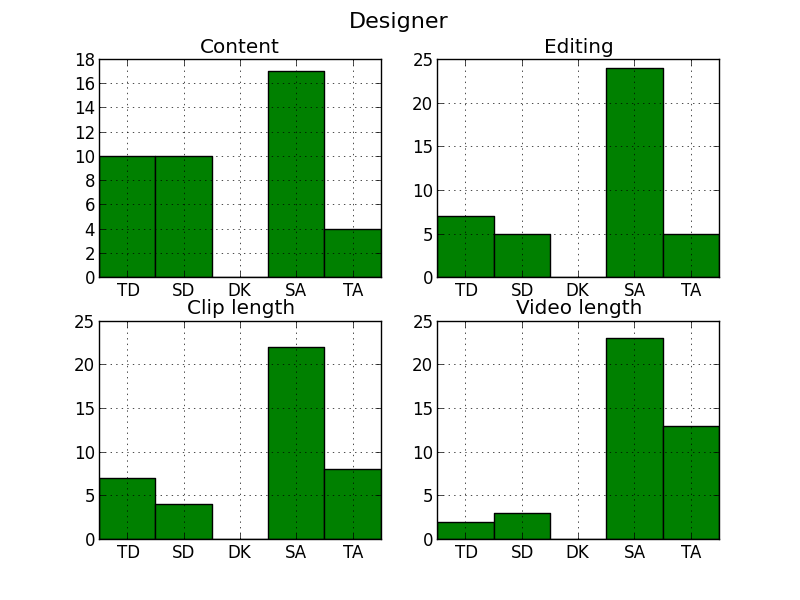
\includegraphics[width=1.0\textwidth]{img/designer_barplot.png}
     \caption{Histogram of answers to videos created with the "designer method"}\label{fig:hist_design}
\end{figure}\\
%
\subsubsection{Friedman Test}
%
% ANDERS
FORMULER NULL HYPOTHESIS\\ %ANDERS
%
We continue our analysis by employing the Friedman rank sum test which is a non-parametric statistical test. We must employ a non-parametric test as parametric tests require the data to follow a specific distribution (the histograms shows that it does not). The values related to each answer are also not compareable value-wise (there is no clear numerical interpretation), ie. \textit{Totally disagree} $(-2)$ is not twice as bad as \textit{Somewhat disagree} $(-1)$, but \textit{Totally disagree} is ranked lower than \textit{Somewhat disagree}. The Friedman test ranks all answers, where answers with equal values get the same rank, and then counts occurence of each rank MORE?. The disadvantage of employing a non-parametric test is that it requires are larger sample size to draw conclusions with the same degree of confidence as a parametric test.\\ 
The results can be found in Tables \ref{tab:fried_alpha}, \ref{tab:fried_dataset}, and \ref{tab:fried_recip} where $\nu$ denotes degrees of freedom, and p-value is \textit{"the probability of obtaining a test statistic at least as extreme as the one that was actually observed, assuming that the null hypothesis is true."}\footnote{http://en.wikipedia.org/wiki/P-value}.\\
% INPUT IS 3 TABLES
\begin{table}[ht]
	\begin{center}
	\caption{Friedman rank sum test for recipies}
	\label{tab:fried_recip}
		\begin{tabular}{lccc}
		\toprule
			 & v & p-value & $x^2$\\
			\midrule
			Content & $3$ & $0.3242$ & $3.4737$\\
			Editing & $3$ & $0.3260$ & $3.4602$\\
			Clip length & $3$ & $0.9597$ & $0.3016$\\
			Video length & $3$ & $0.3218$ & $3.4918$\\
			Total score & $3$ & $0.4882$ & $2.4292$\\
		\bottomrule
		\end{tabular}
	\end{center}
\end{table}
\begin{table}[ht]
	\begin{center}
	\caption{Friedman rank sum test for datasets}
	\label{tab:fried_dataset}
		\begin{tabular}{lccc}
		\toprule
			 & v & p-value & $x^2$\\
			\midrule
			Content & $2$ & $0.0773$ & $5.1193$\\
			Editing & $2$ & $0.5436$ & $1.2190$\\
			Clip length & $2$ & $0.0577$ & $5.7059$\\
			Video length & $2$ & $0.2030$ & $3.1887$\\
			Total score & $2$ & $0.1185$ & $4.2656$\\
		\bottomrule
		\end{tabular}
	\end{center}
\end{table}
\begin{table}[ht]
	\begin{center}
	\caption{Friedman rank sum test for $\alpha$-span}
	\label{tab:fried_alpha}
		\begin{tabular}{lccc}
		\toprule
			 & v & p-value & $x^2$\\
			\midrule
			Content & $1$ & $0.7055$ & $0.1429$\\
			Editing & $1$ & $1.0000$ & $0.0000$\\
			Clip length & $1$ & $0.4652$ & $0.5333$\\
			Video length & $1$ & $0.7055$ & $0.1429$\\
			Total score & $1$ & $0.5271$ & $0.4000$\\
		\bottomrule
		\end{tabular}
	\end{center}
\end{table}
%
Table \ref{tab:fried_recip} shows the result from videos generated by the each method, Table \ref{tab:fried_dataset} shows the results from videos partitioned by video-footage a given video is generated from, and Table \ref{tab:fried_alpha} shows the effect of different $\alpha$-span values (described in section \ref{sec:})
%
\subsubsection{Notes}
%
% ANDERS
PRESENT QUEST. NOTES (need to extract these first)
%
\subsection{Analysis}
%
The only statistical significance is \textit{content} in Table \ref{tab:fried_dataset}. As everything else is statistically insignificant we do not pursue further analysis KIM: VI SKAL LIGE SNAKKE OM HVAD VI GØR HER.
%
\subsection{Risks \& Limitations}
%
User based tests are inherently risky. Our choice of statements and options are bound to have had a huge influence on the results. As is the choice of supporting two languages. Based on feedback from users (both through the test and in person) we have come to understand that several things could have been done better. Several users complained over the lack of context in which they were watching the video. They claimed, rightfully, that it is almost impossible to determine whether clips were interresting or whether the length of a video is fitting, when they did not know what they were watching. The lack of sound only makes this more difficult.\\\\
%
Lots more here...
% LAUGE
% limited dataset -> we did not have seperate training and test sets\\     <- Skal stå i forrige sektion
% barely acceptable amount of feedback -> could have caused ...
% search keywrod kunne måske have hjulpet på at forstå spøgsmål bedre.
%
\section{Summary}
%
% LAUGE

%
% ANDERS
As we are unable to reject the null hypothesis in almost all regards we conclude that the questionaires reveal no significant effect of the various methods of generating a the resulting video. This also means that there is no significant measureable difference between a human edited video and one that is generated at random.\\
There is also no significant measureable effect of choosing different $\alpha$-values, ref to section with alpha-values explained. We only tested for two different values to keep the number of test videos at a manageable level.\\
There was also no significant measureable difference between the three datasets, except in content which is no surprise as the datasets differ primarily on content as described in section \ref{section that describes datasets}.\\
%
We believe that this is an effect of high quality raw material, and we would suspect that there would be a noticeable difference if our dataset had contained a larger amount of video footage of questionable quality; visual, contextual, or both.\\
which leads us to conclude that we must test for values closer to the extreme to get a definite answer. FURTHER ANALYSIS COULD BE TO INVESTIGATE THE EFFECT OF ALPHA VALUES, IE. FOR ALPHA VALUE X WE GET A TOTAL AVR. VIDEO LENGTH OF SO AND SO SECONDS, AND SEGMENT LENGTHS OF SO AND SO SECONDS, COMPARE THAT TO AN ALPHA VALUE OF 2X.\\
%
\chapter{Discussion}
%
% labeling was so dependant on image quality that the quality assesment was not as much needed (other than optimizations we did not perform)
% impact of generally high quality videos (pre-edited and then cut up)
% gold standard is somewhat error prone
%
\chapter{Conclusions}
%
% \section{Summary}\label{sec:conc_summary}
%
Brief summary of the thesis
%
\section{Conclusions}\label{sec:conc_concs}
%
% Explain the current state-of-the-art on the topic of automatic construction of videos 
% -> Uncover the current state-of-the-art on the topic of automatic video summaries from multiple sources
Our first research goal was to uncover the current state-of-the-art on the topic of automatic video summaries from multiple sources. Girgensohn et al.\cite{Girgensohn:2000:SAH:354401.354415} describes a method for a semi-automatic way of editing home video, in which they use automated video analysis to identify suitable clips. However they do not perform any contextual analysis of the footage.
\\\\
% Select, possibly extend, and implement a method for segmenting video clips.
Our image quality assessment was based on methods presented by Girgensohn et al.\cite{Girgensohn:2000:SAH:354401.354415} who proposes a simple and effective way of detecting camera movement frame-by-frame by computing a vector describing the direction and magnutide of the movement. They also proposed a method of detecting overly dark images, on which we improved to also detect overly bright images, or images with little texture such as extreme closeups.\\
We proceeded with different approaches to classifying a single frame of video footage and compare the classification to a gold standard. Several of our approaches provided satisfactory results, but we do question the way we achived the gold standard as this included manual viewing of the entire dataset by one or more human observers and recording their subjective X. OMFORM!\\
% Develop and implement a method for labeling video segments.
We successfully labeled video footage based on a contextual analysis. The analysis was based on metadata from the image quality assesment, and metadata computed for the purpose of labelling. We were able to identify public speakers, footage shot from within a crowd, detect police blinker lights, and overview shots. 
\\
The correctness of each type of label varies, but the \emph{Person in Focus}-label was correct $X\%$ of the time. Other labels such as the \emph{Vertical Oscillation} bla bla. skriv mere om dette. SKAL BRUGE DISSE TAL!
\\\\
% Develop and implement a method for composing a coherent video summary by aggregating video segments. 
% -> Develop a method for composing a video summary from multiple sources with a coherent contextual flow
When we had completed labelling the video footage we moved on to creating the video summaries. We used a cooking analogy where a recipe is a list of ingredients, in a specific order, each defining a type of footage, that we would like to include in the final video. For each ingredient we try to find the most fitting sub-part of a video that matches the description of the ingredient, where the ingredient would be a list of parameters such as labels required and how long the part should be. For this purpose we designed an algorithm that computes a score for each sub-part based on an input ingredient and available footage.\\
We initially had plans of using machine learning for creating the summary, but this would require extensive training, possibly involving external feedback, and simply would not fit within the scope of the project.
\\\\
% Evaluate the final architecture and prototype with respect to domain-specific metrics (primarily focusing on quality and processing time)
The inspiration for this project based on an idea of a service that would process live video-streaming into a live video-summary. Such a service impose a low treshold on processing time for each video-stream. Image quality assessment is achiveable during playback and provides a good base for later optimization as we experienced that contextual analysis is mostly fruitless when performed on video footage of questionably quality. Ie. contextual analysis is only strictly needed on high quality footage, and an efficient approach as such. Object detection was one of the most ressource consuming processes, although capable of a live-analysis, we attempted to detect multiple objects (face, profile, and upper body), making multi-processing an absolute must. Most research the area of object detection in images is focused on still images, but research does exist on ex. detecting cars in traffic. We expect it to only be a matter of time before we see object detection optimized for video.
% Sum it up ?

%
\section{Limitations}\label{sec:conc_lims}
%
\section{Future Work}\label{sec:futurework}
%
% KIM: 60 kommentarer til denne section
Had we had our own video hosting service we would have access to such information.Had we further had our own client application in which all video was recorded we would even be able to acquire additional information about the circumstances in which the footage was recorded. Examples of this could be information about the movement of the camera (from accelerometers) and proximity to other devices recording the same scene (through Bluetooth). The purpose of our method for building our dataset has been to simulate that we do in fact have access to some of this information, as well as making it as easy as possible to estimate the rest.
%
image quality in a live system\\
more extreme alpha span value
%
\newpage
\appendix
%
% \section{Histograms}\label{app:histograms}

\bibliographystyle{plain}
\bibliography{references}
\end{document}